\documentclass [aspectratio=169]{beamer}
\beamertemplatenavigationsymbolsempty
\usetheme{Boadilla}
\usepackage{textpos} % package for the positioning
\usepackage[]{graphicx}
\usepackage{graphicx}
\usepackage{float}
\usepackage{hyperref}
\usepackage{caption}
\usepackage{subcaption}
\usepackage{algorithm,algpseudocode}
\usepackage[export]{adjustbox}
\usepackage{tikz}
\usepackage[square,numbers]{natbib}
\usepackage[byname]{smartref}
\usetikzlibrary{positioning}
\usetikzlibrary{arrows, shapes, decorations, automata, backgrounds, fit, petri, calc}

\newcommand*{\logofont}{\fontfamily{phv}\selectfont}

\definecolor{uwopurple}{RGB}{79,38,131} % official purple color for uwo

\title[]{\vspace{60pt} \\
Sailing to Ithaca} % Change the lecture topic right here!
\subtitle{The road to normal hierarchy}
\author[]{J.J. Gómez Cadenas}
\institute[]{Donostia International Physics Center}
\date{\today}

% Math notations
\newtheorem{thm}{Theorem}[section]
\newtheorem{lem}[thm]{Lemma}

\newtheorem{defn}[thm]{Definition}
\newtheorem{eg}[thm]{Example}
\newtheorem{ex}[thm]{Exercise}
\newtheorem{conj}[thm]{Conjecture}
\newtheorem{cor}[thm]{Corollary}
\newtheorem{claim}[thm]{Claim}
\newtheorem{rmk}[thm]{Remark}

\newcommand{\ie}{\emph{i.e.} }
\newcommand{\cf}{\emph{cf.} }
\newcommand{\into}{\hookrightarrow}
\newcommand{\dirac}{\slashed{\partial}}
\newcommand{\bbonu}{\ensuremath{\beta\beta0\nu}}
\newcommand{\bbtnu}{\ensuremath{\beta\beta2\nu}}
\newcommand{\mbb}{\ensuremath{m_{\beta\beta}}}
\newcommand{\qbb}{\ensuremath{Q_{\beta\beta}}}
\newcommand{\mbbsq}{\ensuremath{m_{\beta\beta}^2}}
\newcommand{\tonu}{\ensuremath{(T_{1/2}^{0\nu})^{-1}}}
\newcommand{\gonu}{\ensuremath{G^{0\nu}}}
\newcommand{\monu}{\ensuremath{| M^{0\nu}|^2}}
\newcommand{\XE}{\ensuremath{{}^{136}{\rm Xe}}}
\newcommand{\XES}{\ensuremath{{}^{137}{\rm Xe}}}
\newcommand{\GE}{\ensuremath{{}^{76}{\rm Ge}}}
\newcommand{\TE}{\ensuremath{{}^{130}{\rm Te}}}
\newcommand{\TL}{\ensuremath{{}^{208}{\rm Tl}}}
\newcommand{\BI}{\ensuremath{{}^{214}{\rm Bi}}}
\newcommand{\MO}{\ensuremath{{}^{100}{\rm Mo}}}
\newcommand{\KR}{\ensuremath{{}^{83}{\rm Kr}}}
\newcommand{\nne}{\ensuremath{\bar{N}_e}}
\newcommand{\nng}{\ensuremath{\bar{N}_\gamma}}
\newcommand{\so}{\ensuremath{\rm S_1}}
\newcommand{\st}{\ensuremath{\rm S_2}}
\newcommand{\tz}{\ensuremath{\rm t_0}}
\newcommand{\R}{\mathbb{R}}
\newcommand{\C}{\mathbb{C}}
\newcommand{\Z}{\mathbb{Z}}
\newcommand{\N}{\mathbb{N}}
\newcommand{\Q}{\mathbb{Q}}
\newcommand{\LieT}{\mathfrak{t}}
\newcommand{\T}{\mathbb{T}}
\newcommand{\A}{\mathds{A}}
\newcommand{\E}{\mathbb{E}}
\newcommand{\Prob}{\mathbb{P}}
\newcommand{\Var}{\text{Var}}
\newcommand\equalhat{%
\let\savearraystretch\arraystretch
\renewcommand\arraystretch{0.3}
\begin{array}{c}
\stretchto{
    \scalerel*[\widthof{=}]{\wedge}
    {\rule{1ex}{3ex}}%
}{0.5ex}\\ 
=%
\end{array}
\let\arraystretch\savearraystretch
}

% set color
\setbeamercolor{title in head/foot}{bg=white}
\setbeamercolor{author in head/foot}{bg=white}
\setbeamercolor{date in head/foot}{fg=uwopurple}
\setbeamercolor{date in head/foot}{bg=white}
\setbeamercolor{title}{fg=uwopurple}
\setbeamerfont{title}{series=\bfseries}
\setbeamercolor{frametitle}{fg=uwopurple}
\setbeamerfont{frametitle}{series=\bfseries}
\setbeamercolor{block title}{bg=uwopurple!30,fg=black}
\setbeamercolor{item}{fg=uwopurple}
\setbeamercolor{caption name}{fg=uwopurple!70!}


% set logo at non-title pages
%\logo{
\includegraphics[height=0.9cm]{dipc.png}\vspace*{-.45\paperheight}\hspace*{.50\paperwidth}}

\begin{document}

{
\setbeamertemplate{logo}{}
\begin{frame}
    \titlepage
    \begin{textblock*}{4cm}(0.5cm,-7.3cm)
        
\includegraphics[width=4cm]{dipc.png}
    \end{textblock*}
    \begin{textblock*}{8cm}(5.0cm,-7.0cm)
        \huge \color{uwopurple}{$\Bigr\rvert$ \hspace{0.15cm} \textbf{Lecture 5}} % Change the lecture # right here! 
    \end{textblock*}
\end{frame}
}

%%%%
\begin{frame}{The Odyssey}
\begin{columns}
\column{0.60\textwidth}
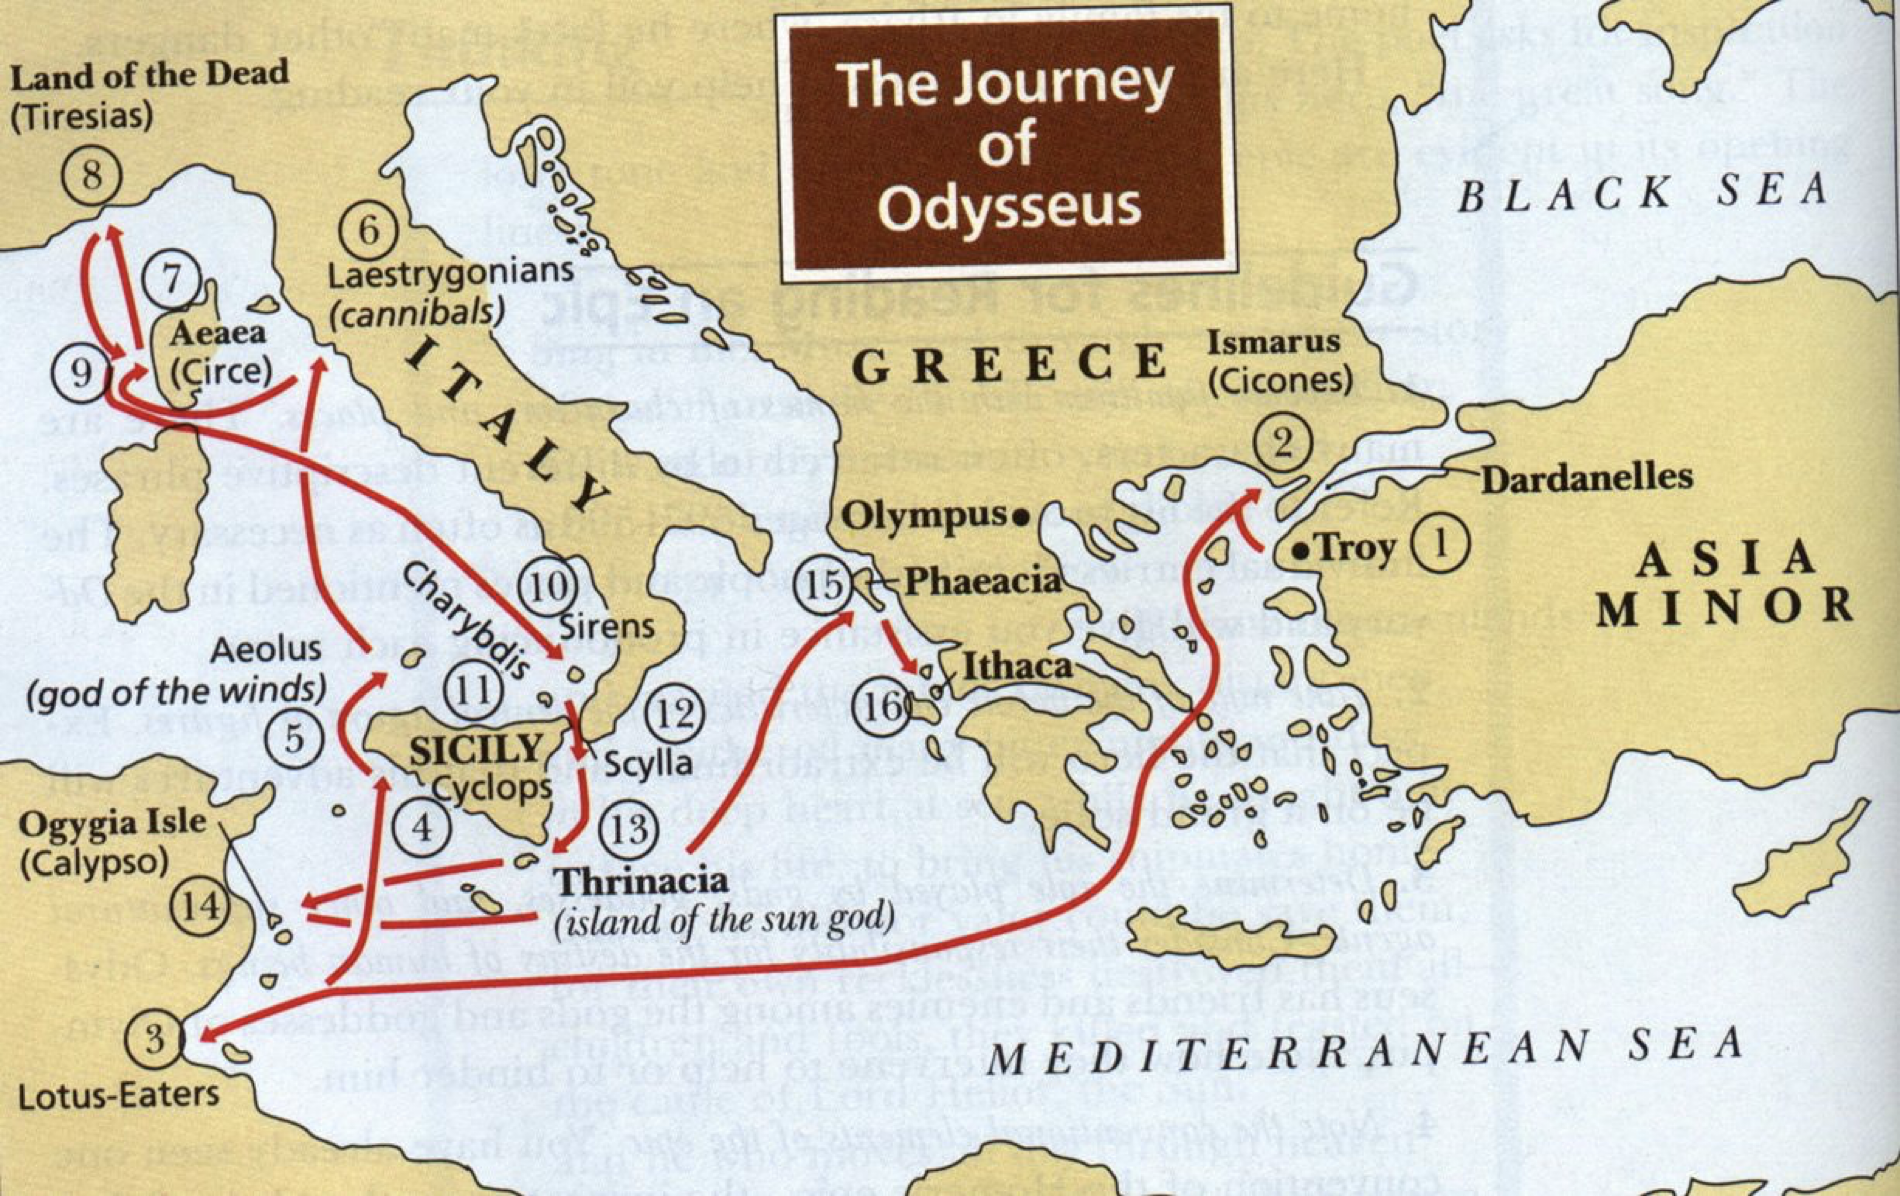
\includegraphics[scale=0.26]{odyssey.png}

\column{0.40\textwidth}
$\bullet~$ The tale of discoveries in (neutrino) physics could be told as odysseys, often involving the long 20 years that Ulysses needs to return to Ithaca. 

$\bullet~$ For example, the Kamioka experiment was commissioned in the early 80’s and by the 2000’s it had dramatically contributed to the discovery of neutrino oscillations. 

\end{columns}
\end{frame}

%%%%
\begin{frame}{Every odyssey starts with a terrific idea}

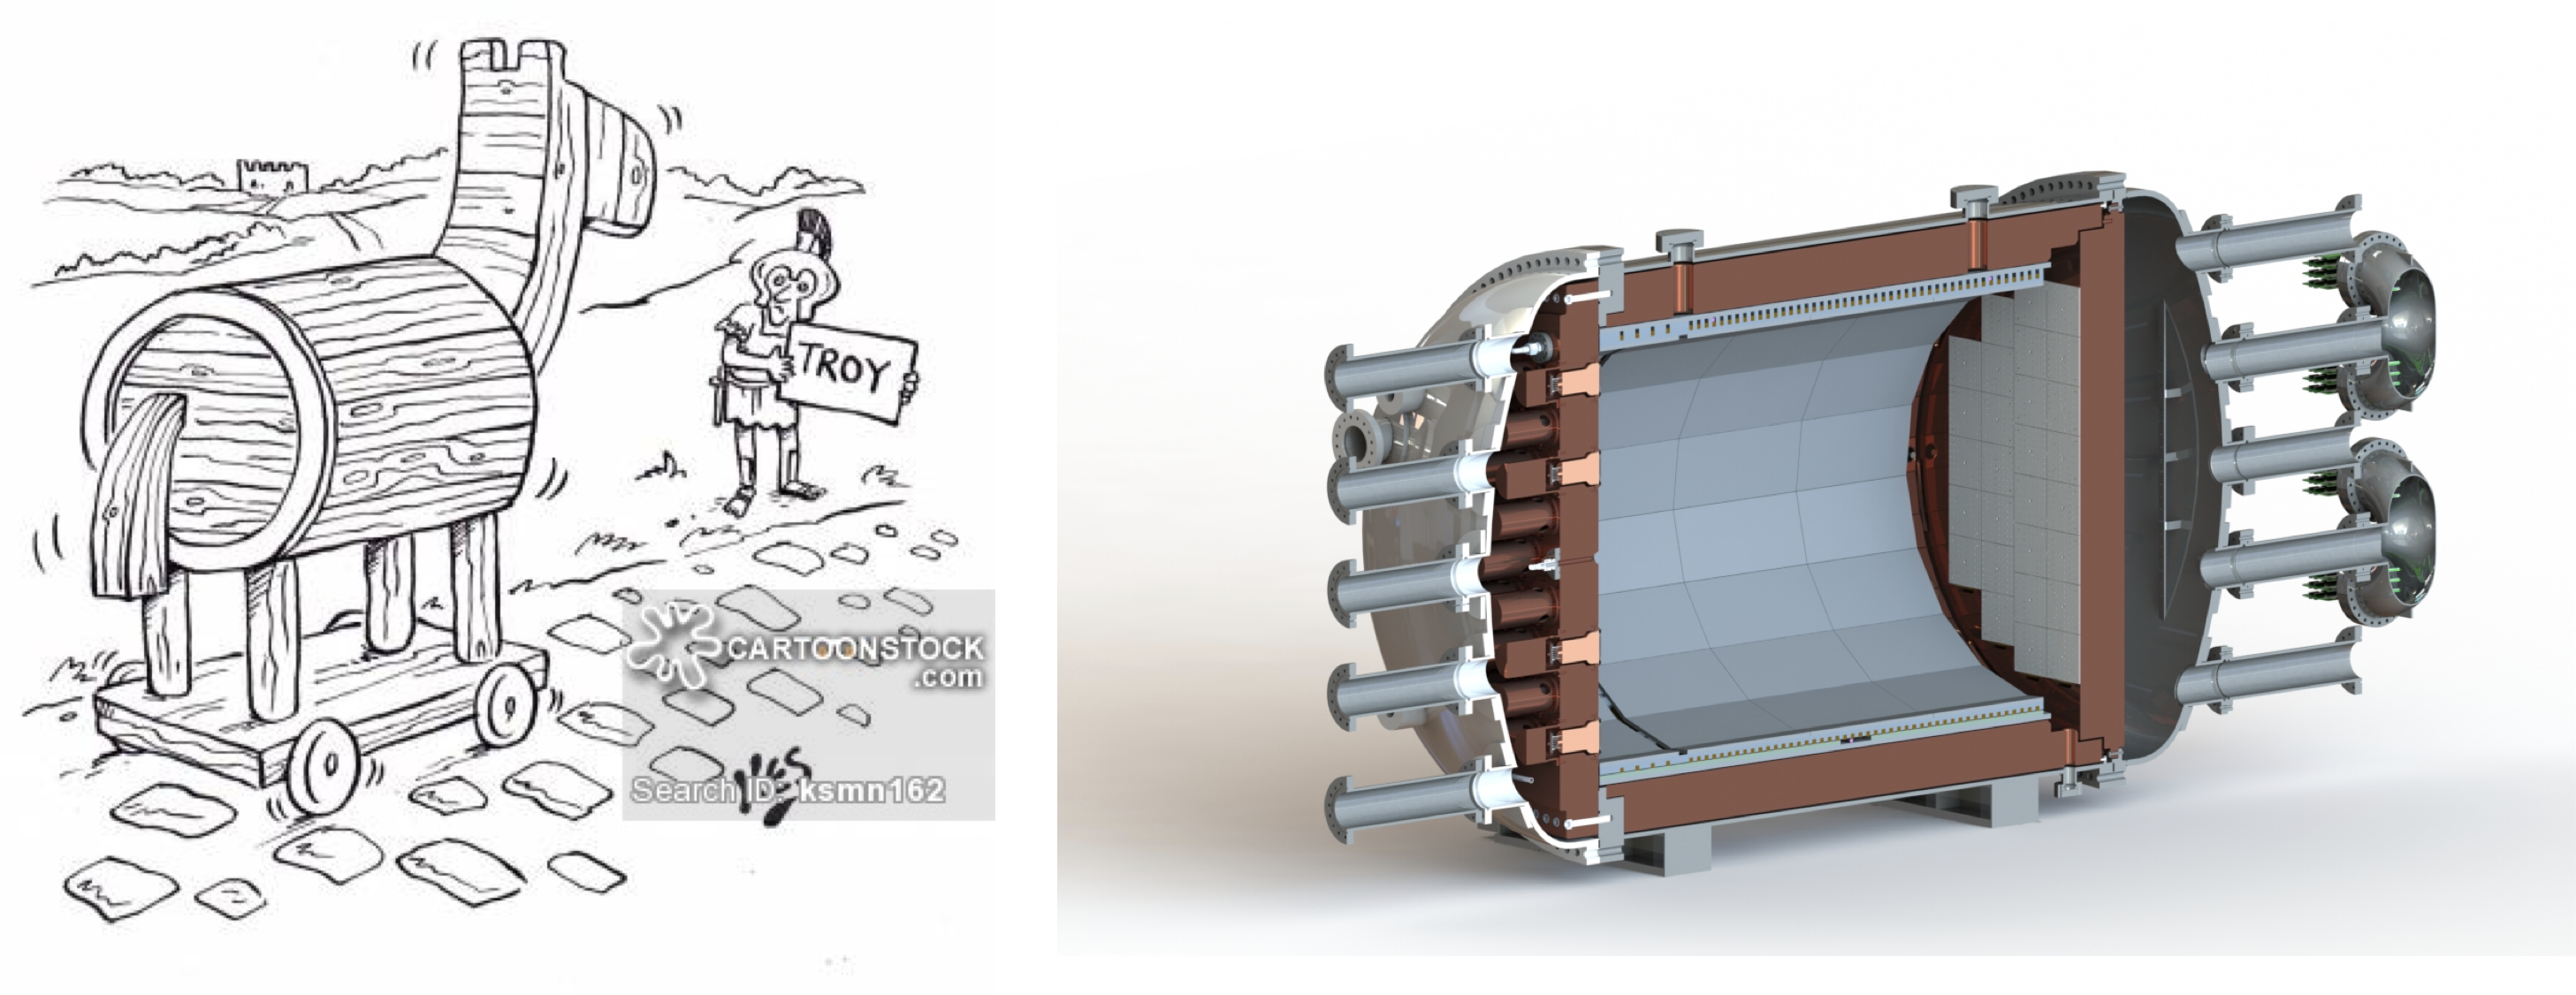
\includegraphics[scale=0.26]{odysseystart.png}

\begin{columns}
\column{0.50\textwidth}

$\bullet~$ A new device to conquer Troy.  

\column{0.50\textwidth}
$\bullet~$ A new device to conquer \bbonu.

\end{columns}

\end{frame}

%%%
\begin{frame}{And utter ignorance of the upcoming complications…}

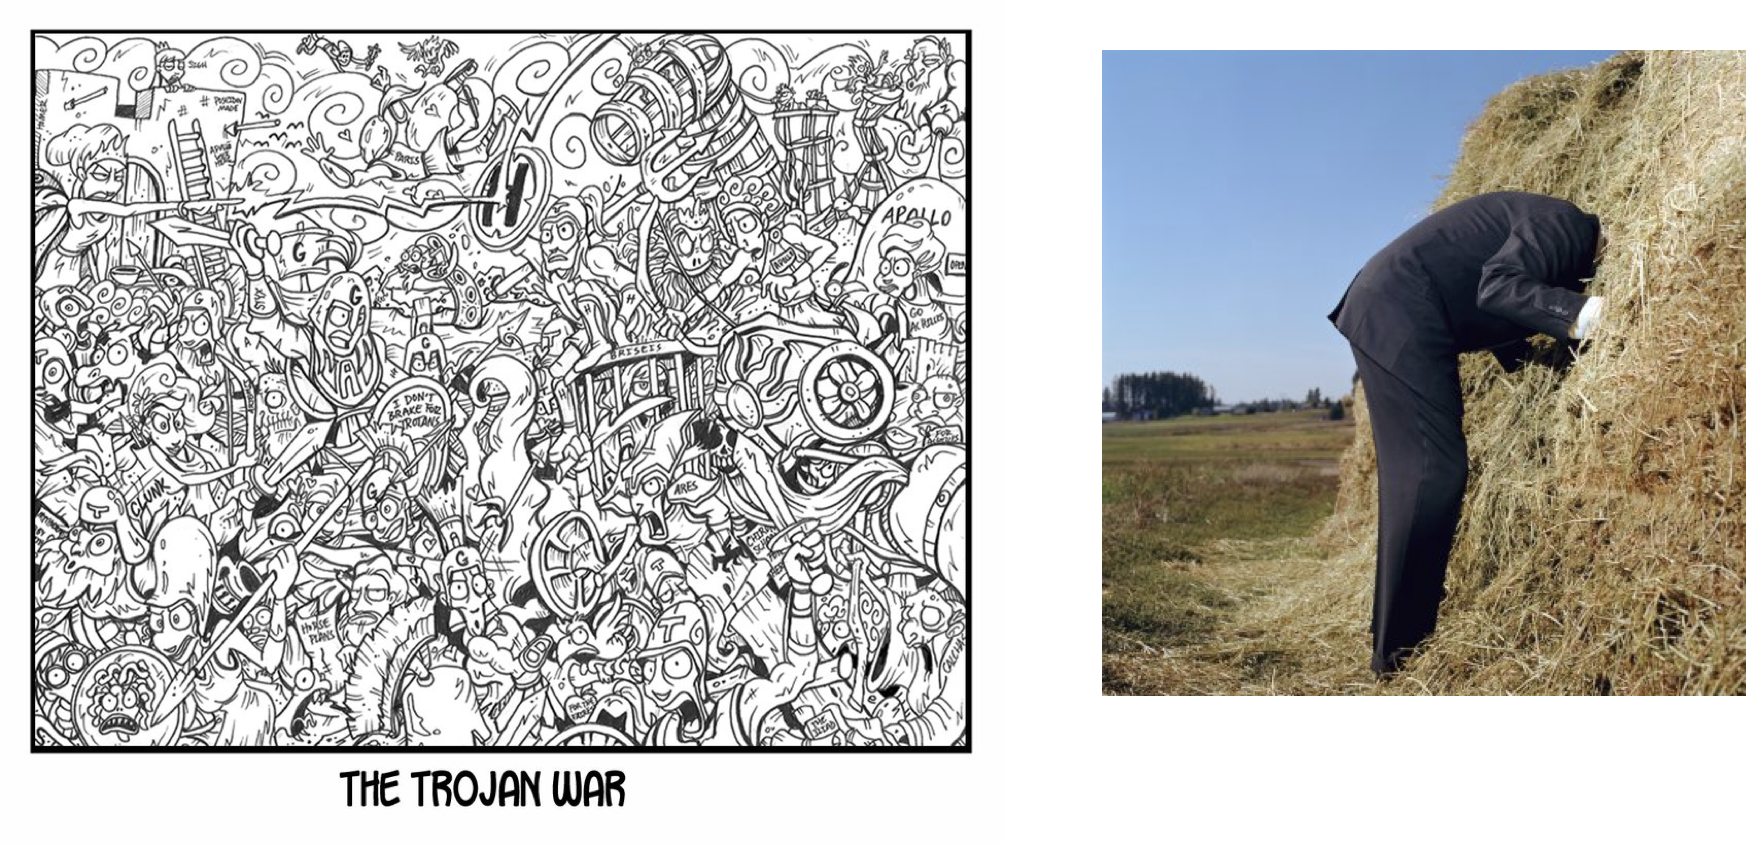
\includegraphics[scale=0.45]{complications.png}

\end{frame}

%%%
\begin{frame}{The Road to Ithaca of the NEXT program (first 20 years)}

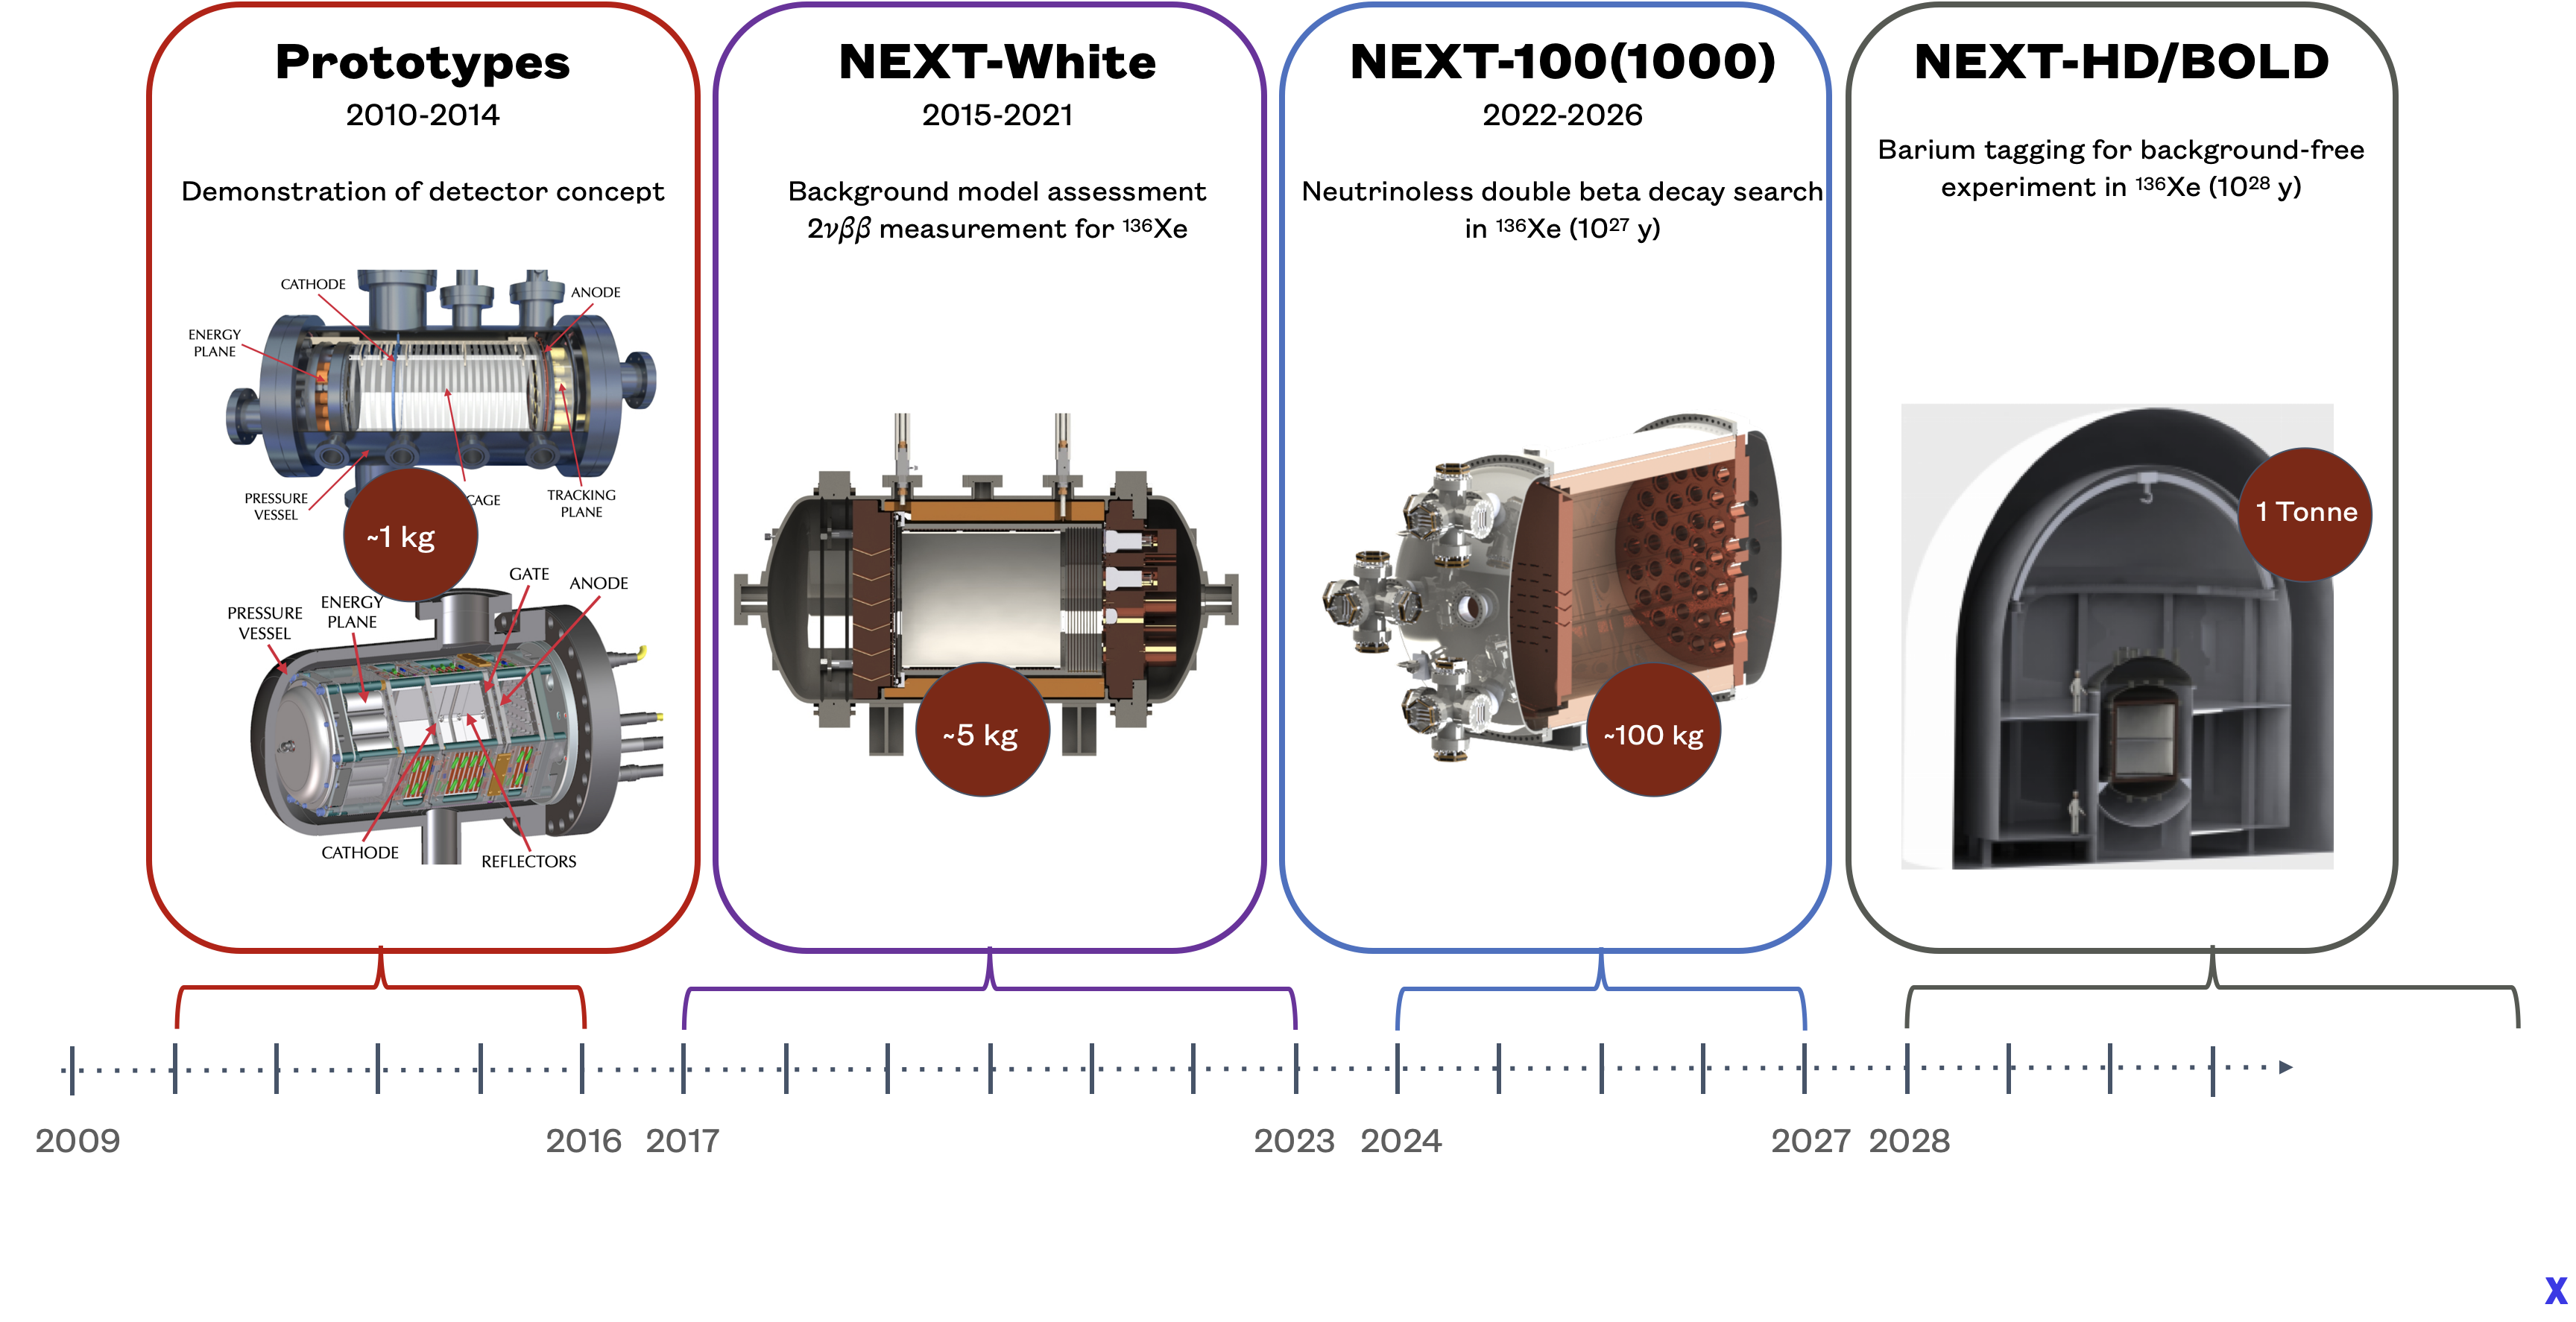
\includegraphics[scale=0.23]{nextprogram.png}

\end{frame}


%%%
\begin{frame}{NEXT-100}

\begin{columns}
\column{0.60\textwidth}
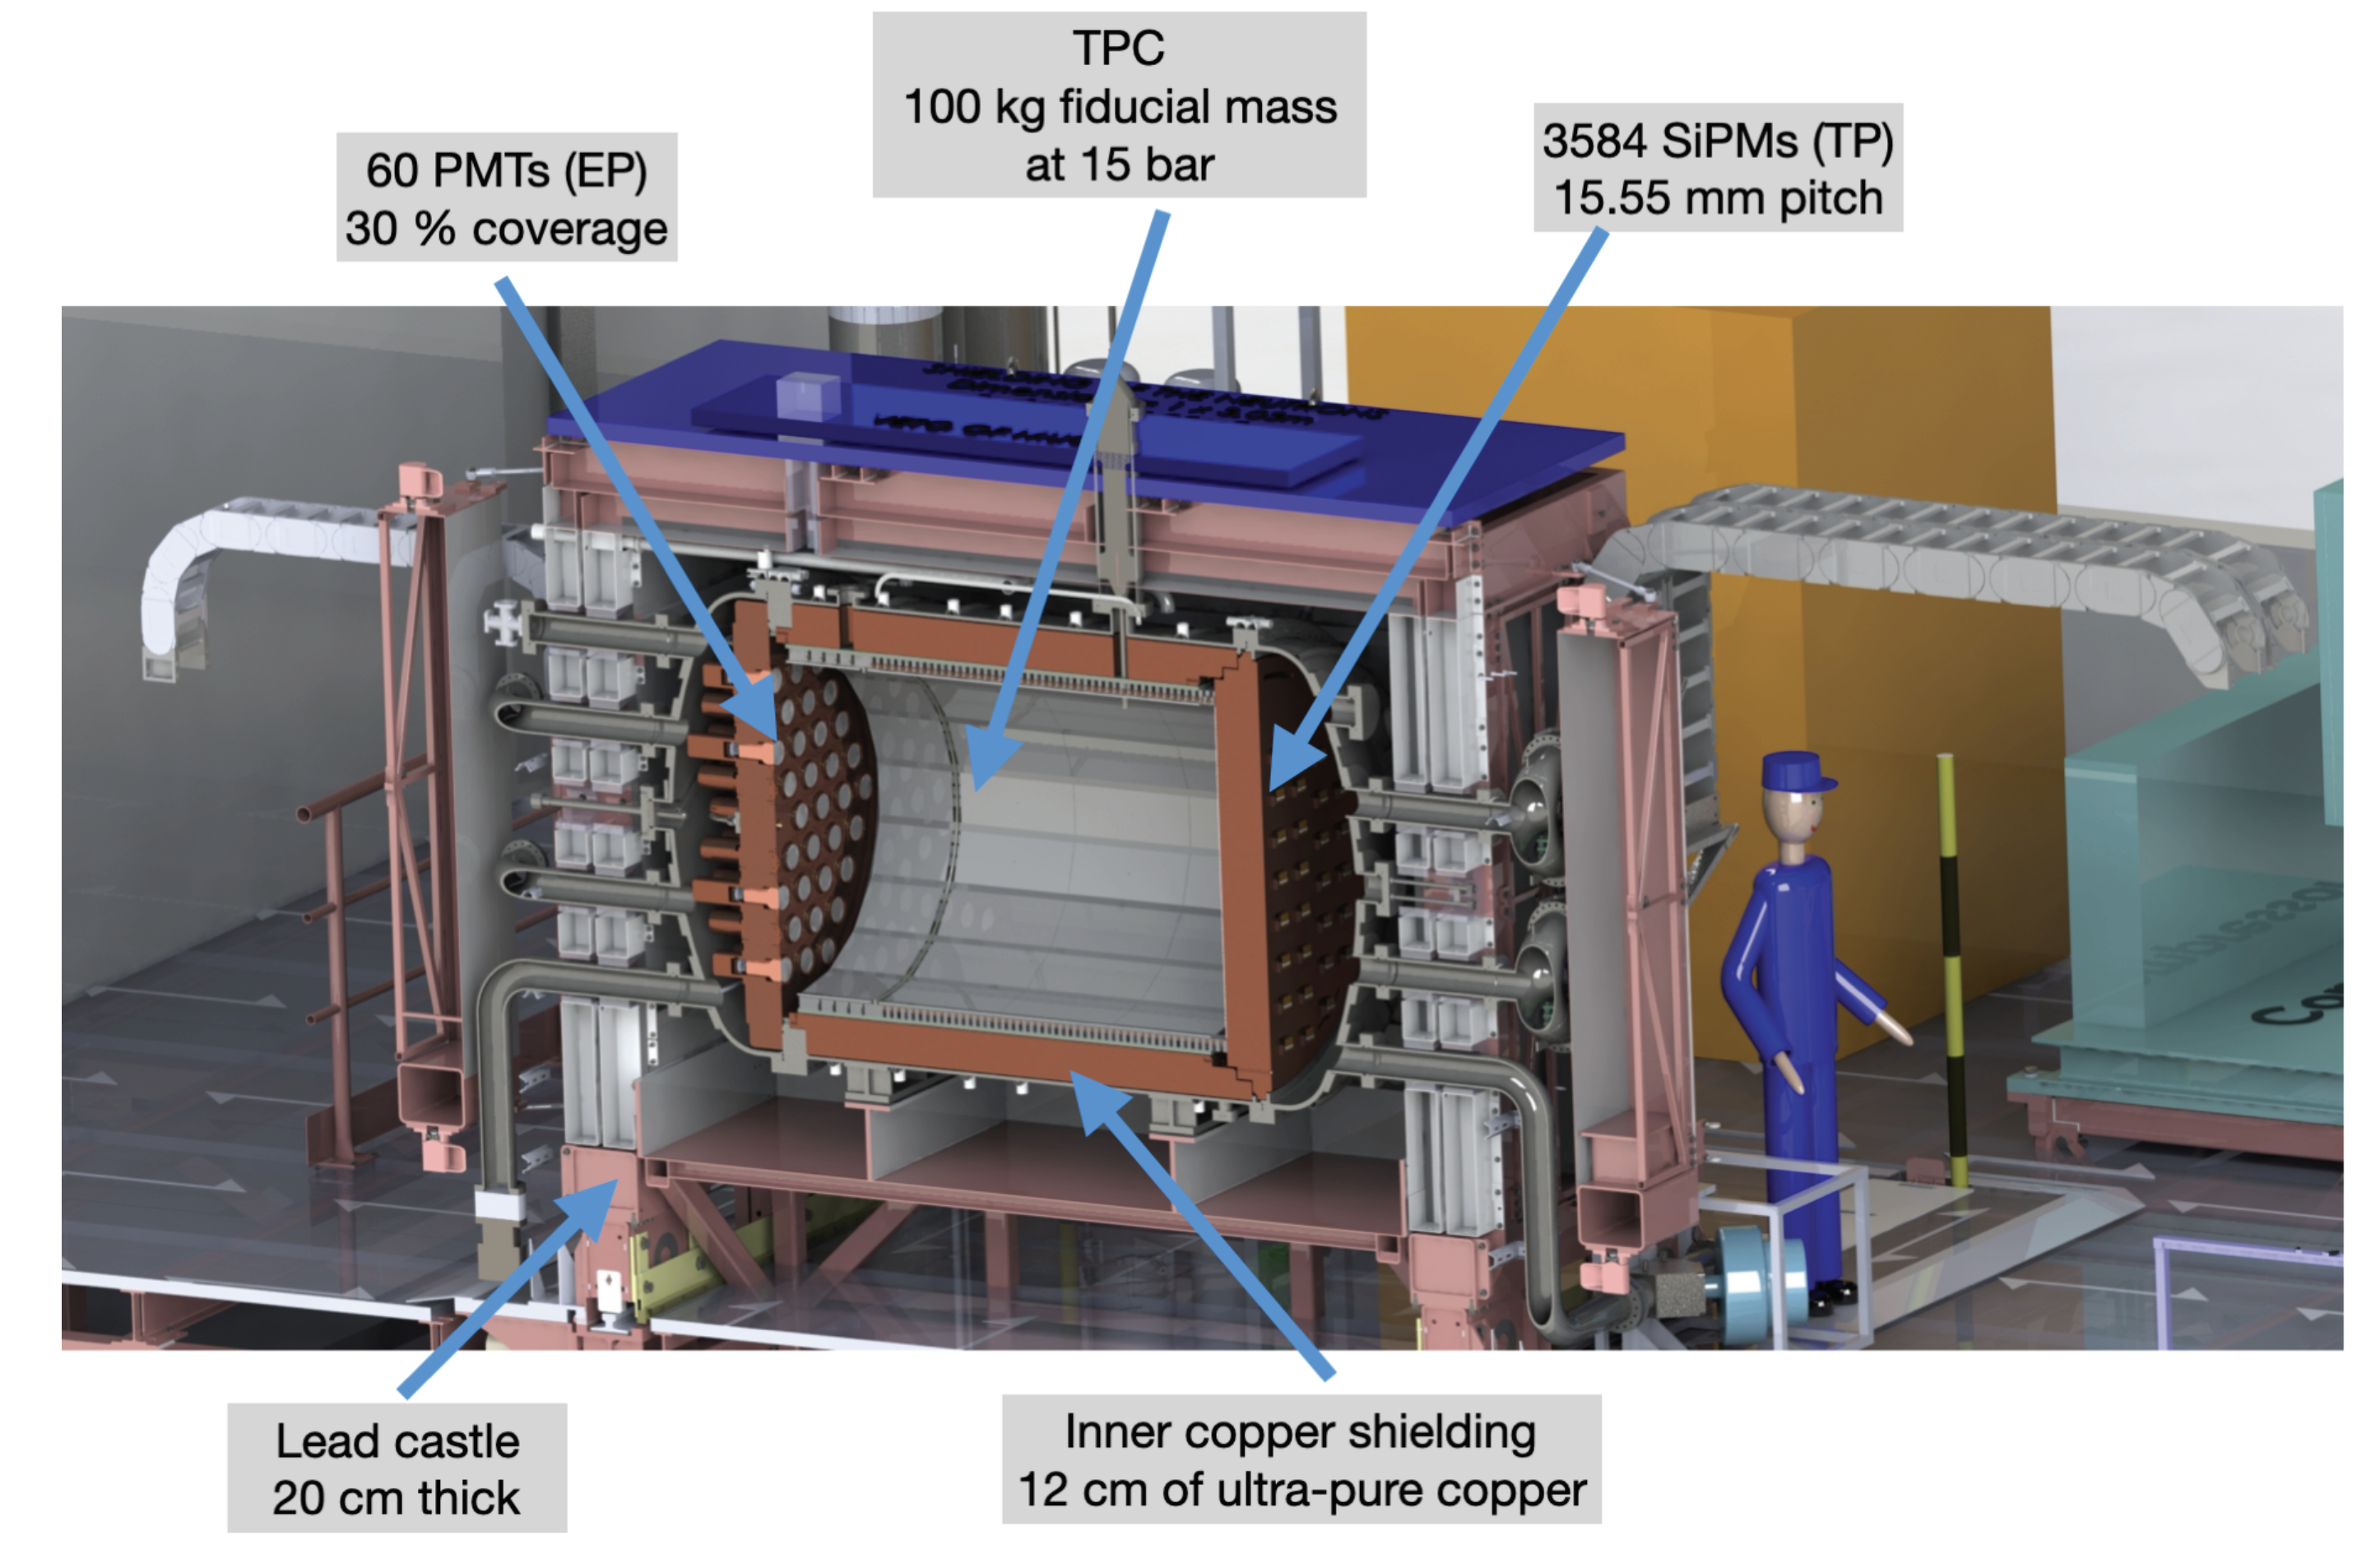
\includegraphics[scale=0.24]{next100withcastle.png}


 \column{0.40\textwidth}
$\bullet~$ NEXT-100 is operating at LSC since 2024. It scales up NEXT-White by a factor 2.2 in dimensions, thus a factor 10 in mass.  

$\bullet~$ Was NEXT-100 necessary? Why not scaling up directly from NEXT-White to ton-class detectors? The answer is very instructive to understand the challenges facing \bbonu\ experiments.

\end{columns}
\end{frame}

%%%
%\begin{frame}{Pressure Vessel and Inner Copper Shield}
%
%\includegraphics[scale=0.23]{pvandics.png}
%
%\end{frame}

\begin{frame}{Lead Castle}

\includegraphics[scale=0.08]{leadCastle.png}

\end{frame}


%%%
\begin{frame}{Pressure Vessel}

\includegraphics[scale=0.23]{next100pv.png}

\end{frame}

%%%
\begin{frame}{Inner Copper Shield}

\includegraphics[scale=0.23]{innercopper.png}

\end{frame}

%%%
\begin{frame}{Anode \& Cathode grids}

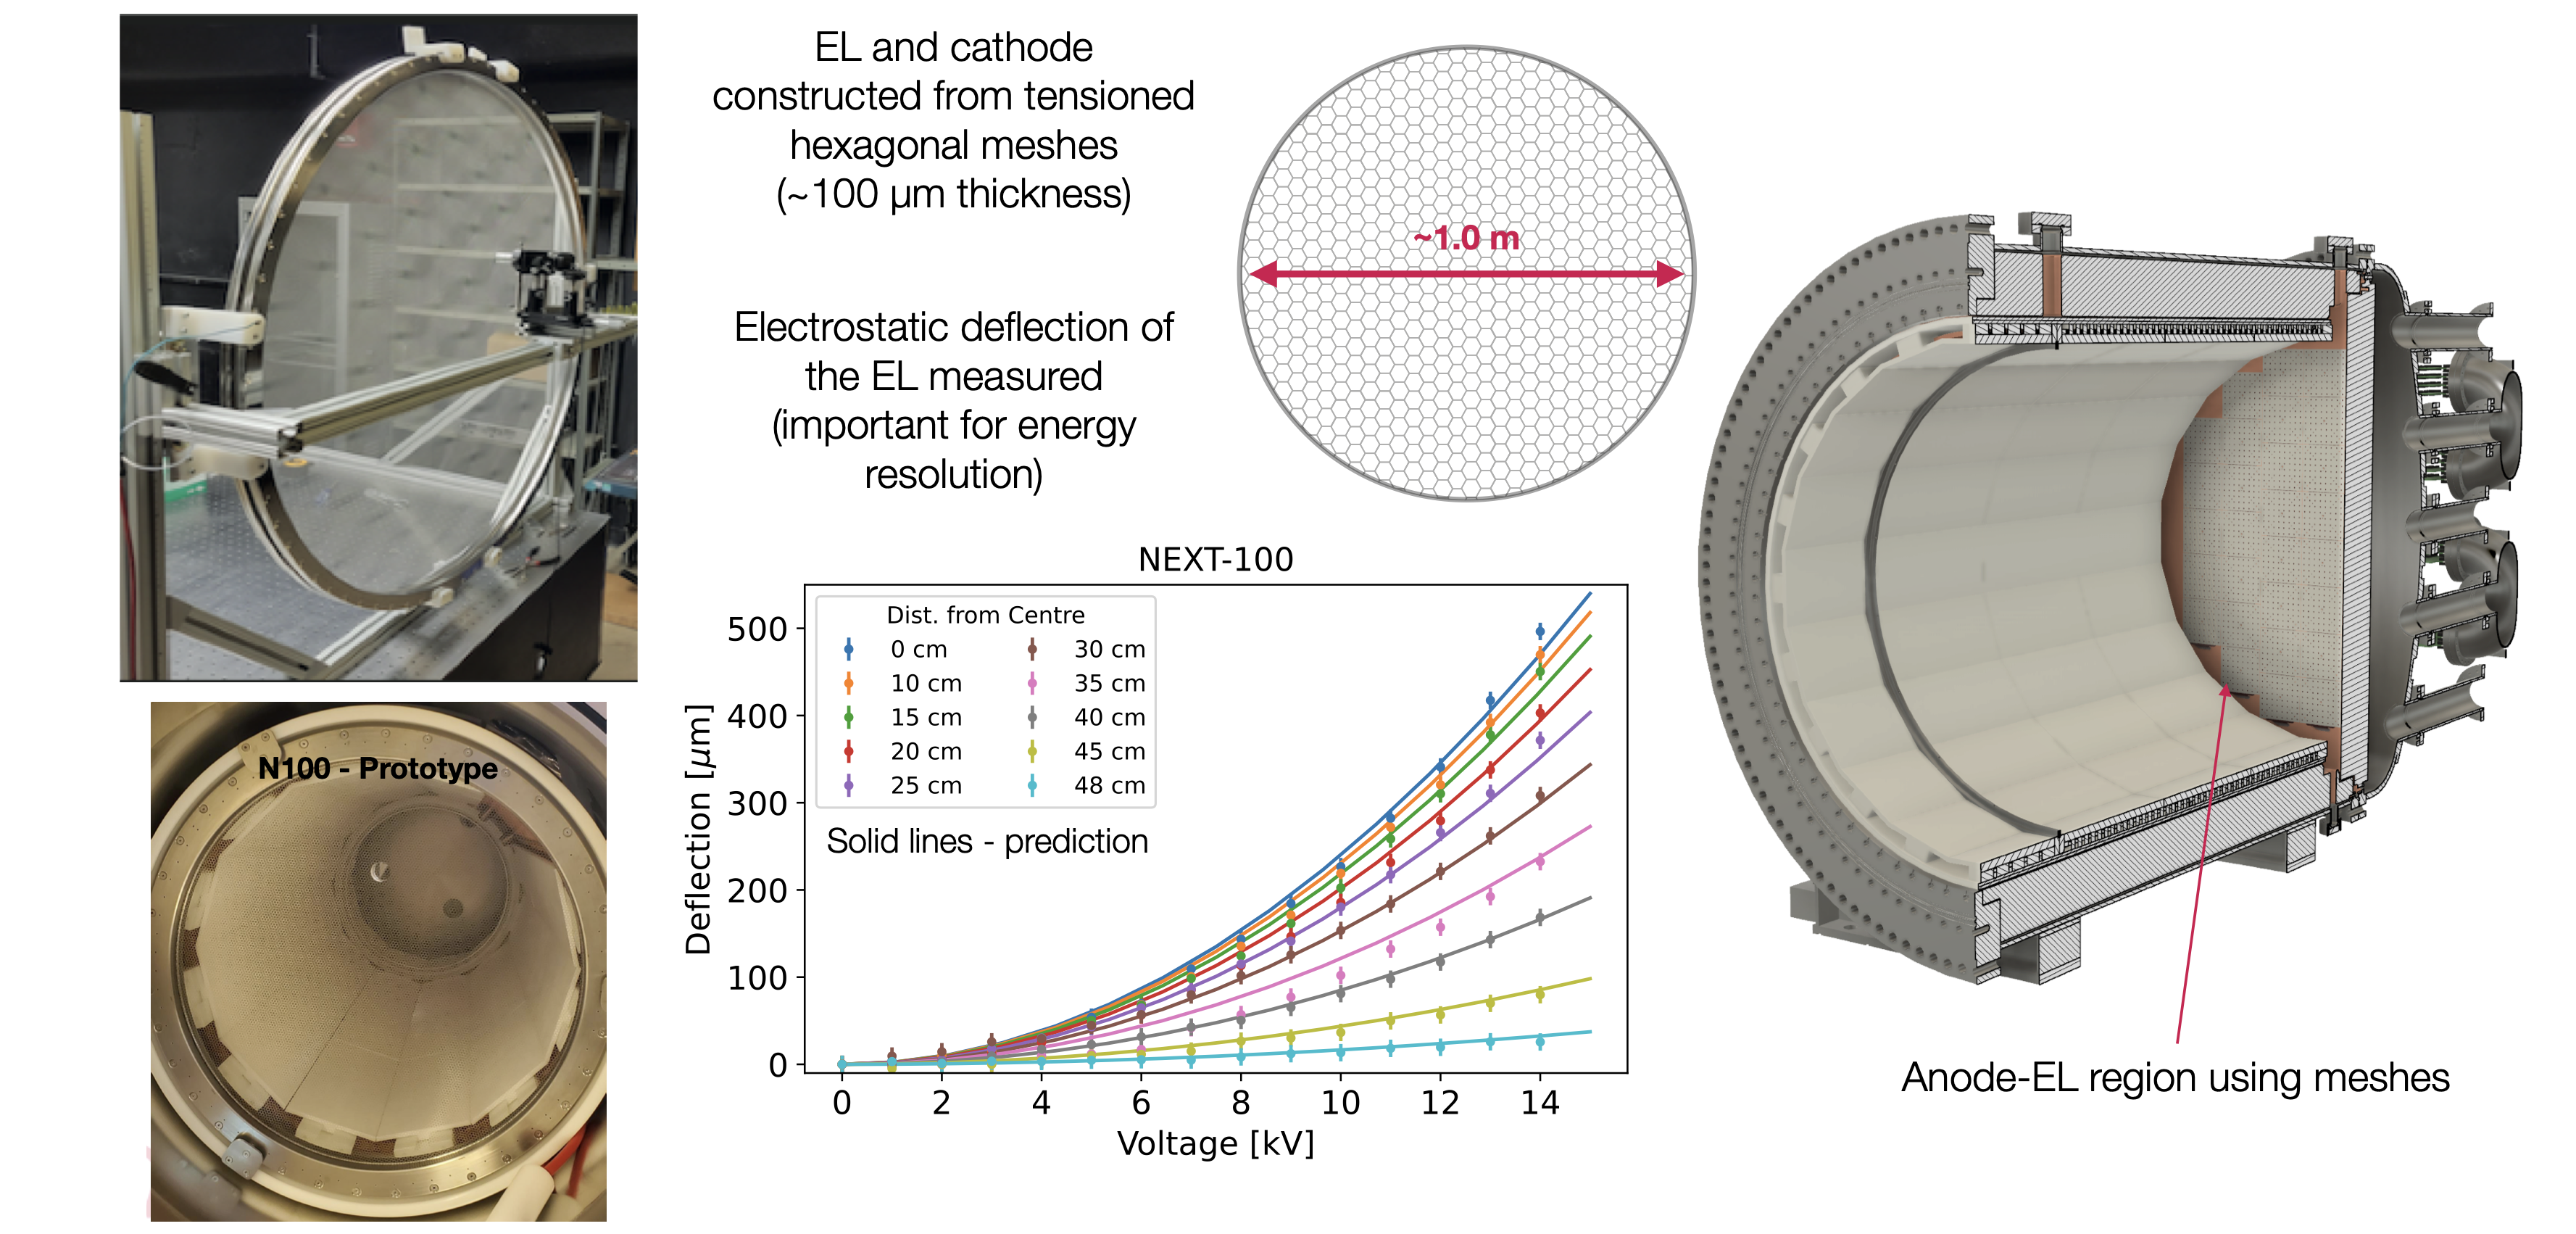
\includegraphics[scale=0.23]{meshes.png}

\end{frame}

%%%

\begin{frame}{Cathode}

\includegraphics[scale=0.21]{cathodeMesh.png}

\end{frame}

%%%

\begin{frame}{PMTs \& SiPMs}

\includegraphics[scale=0.23]{sipmandpmts.png}

\end{frame}

%%%

\begin{frame}{Tracking Plane}

\includegraphics[scale=0.23]{trackingplaneNext100.png}

\end{frame}

%%%%%%
\begin{frame}{Field Cage}

\includegraphics[scale=0.23]{fieldcage.png}

\end{frame}

%%%%%%

\begin{frame}{Light Tube}

\includegraphics[scale=0.21]{LightTube.png}

\end{frame}

%%%%%%

\begin{frame}{Backgrounds: The Matrioska effect}
\begin{columns}
\column{0.50\textwidth}

\includegraphics[scale=0.40]{matrioska.png}

\column{0.50\textwidth}
$\bullet~$ NEXT-100 (and all \bbonu\ experiments) are conceived like Matrioskas, in which the outer shell shields from a higher background and the inner shell shields from the backgrounds passing the outer shells. 

$\bullet~$ In NEXT-100, the Underground Lab shields from cosmics, the Lead Castle shields from the radioactivity of the lab, and the ICS shields the lead castle (and pressure vessel).

$\bullet~$ The radioactive budget comes determined by the last shield (ICS) and the elements in direct contact with the gas (plastics, grids and sensors). 
 \end{columns}
\end{frame}

%%%%%%

\begin{frame}{Backgrounds: The main suspects}
\begin{columns}
\column{0.60\textwidth}
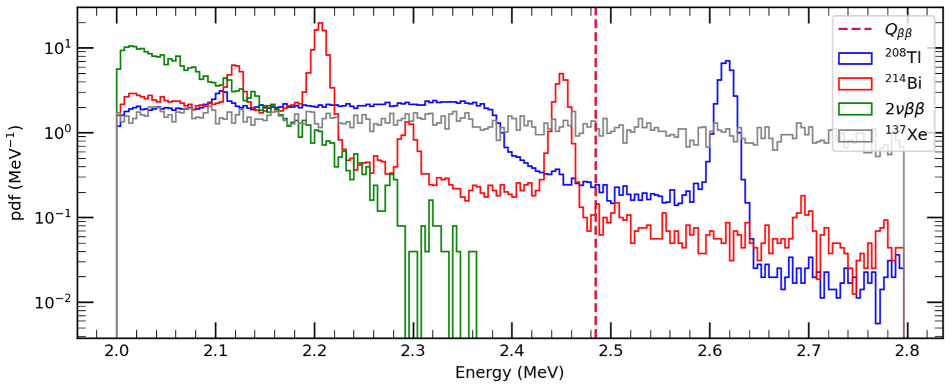
\includegraphics[scale=0.50]{bkgndSpectrum.png}

\column{0.40\textwidth}
$\bullet~$ Natural radioactivity. Gammas from \TL\ ($\sim 2.6$~MeV) and \BI\ ($\sim 2.5$~MeV). Photoelectric peak very near \qbb. 

$\bullet~$ \XES\ activation (depends on the depth of the experiment). 

$\bullet~$ Crossing $\mu$ \& prompt gammas  (depends on the depth of the experiment). 

 \end{columns}
\end{frame}

\begin{frame}{Raw background contributions}
\begin{columns}
\column{0.60\textwidth}
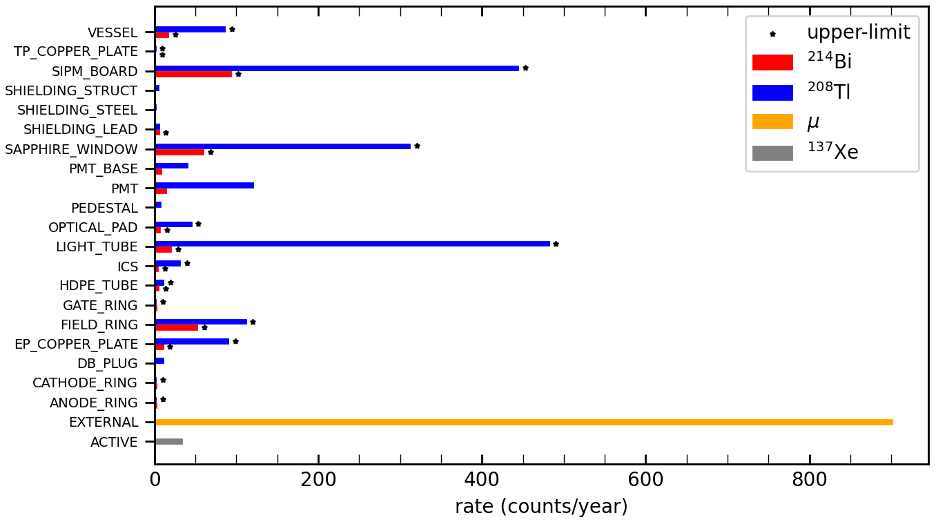
\includegraphics[scale=0.50]{rawBkgnd.png}

\column{0.40\textwidth}
$\bullet~$ Events that deposit energy in the range 2.4-2.5 MeV. 
$\bullet~$(*) marks an upper limit in the measurement of material. For example, the apparent large contribution of the light tube comes from a large upper limit in the activity of teflon. Take with a grain of salt. 

 \end{columns}
\end{frame}

%%%%
\begin{frame}{Background suppression}
\begin{columns}
\column{0.50\textwidth}
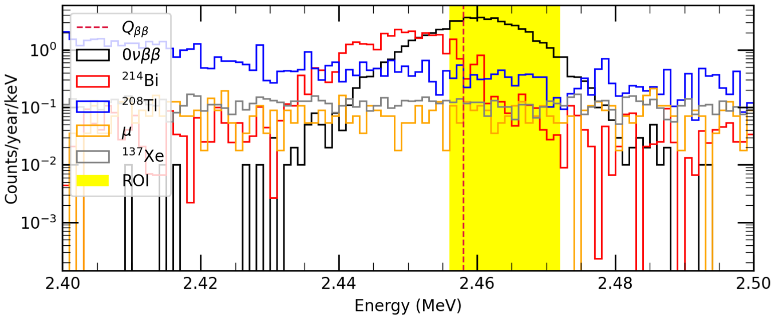
\includegraphics[scale=0.55]{bkgndROI.png}

$\bullet~$ Asymmetric ROI, chosen to maximise $S/\sqrt{B}$ .

\column{0.50\textwidth}
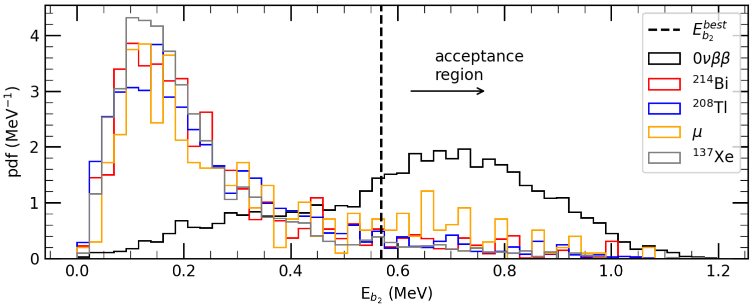
\includegraphics[scale=0.55]{topoSel.png}

$\bullet~$ 70 \% signal efficiency, 91 \% background suppression.

 \end{columns}
\end{frame}

%%%%
\begin{frame}{Background reduction}
\begin{columns}
\column{0.50\textwidth}
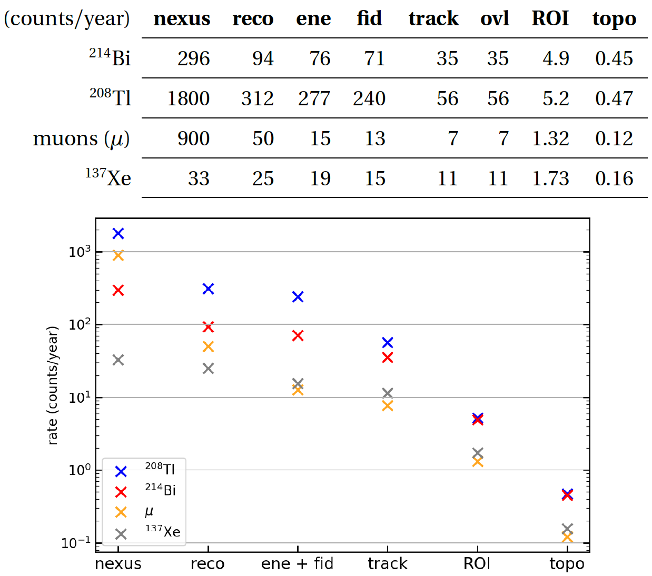
\includegraphics[scale=0.55]{bkgndReduction.png}

\column{0.50\textwidth}
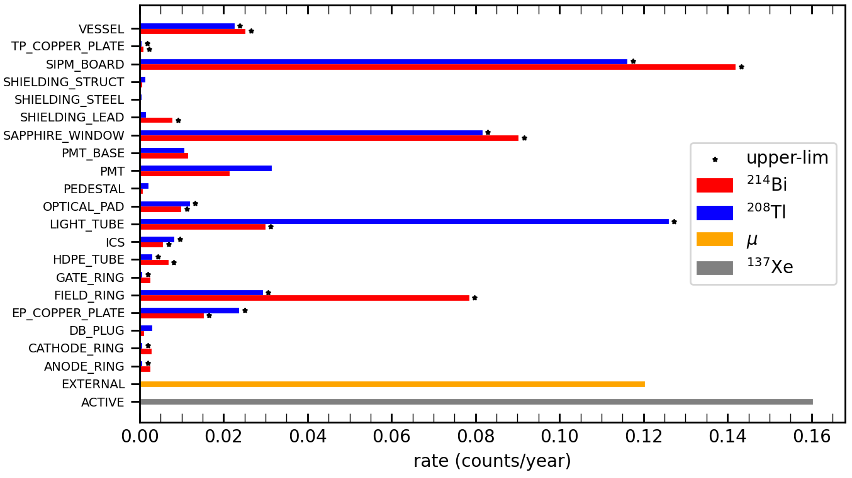
\includegraphics[scale=0.50]{bkgndFinal.png}

$\bullet~$ Background rate: 1.1 counts/year

 \end{columns}
\end{frame}



%\begin{frame}{NEXT-100 Radioactive Budget}
%\begin{columns}
%\column{0.50\textwidth}
%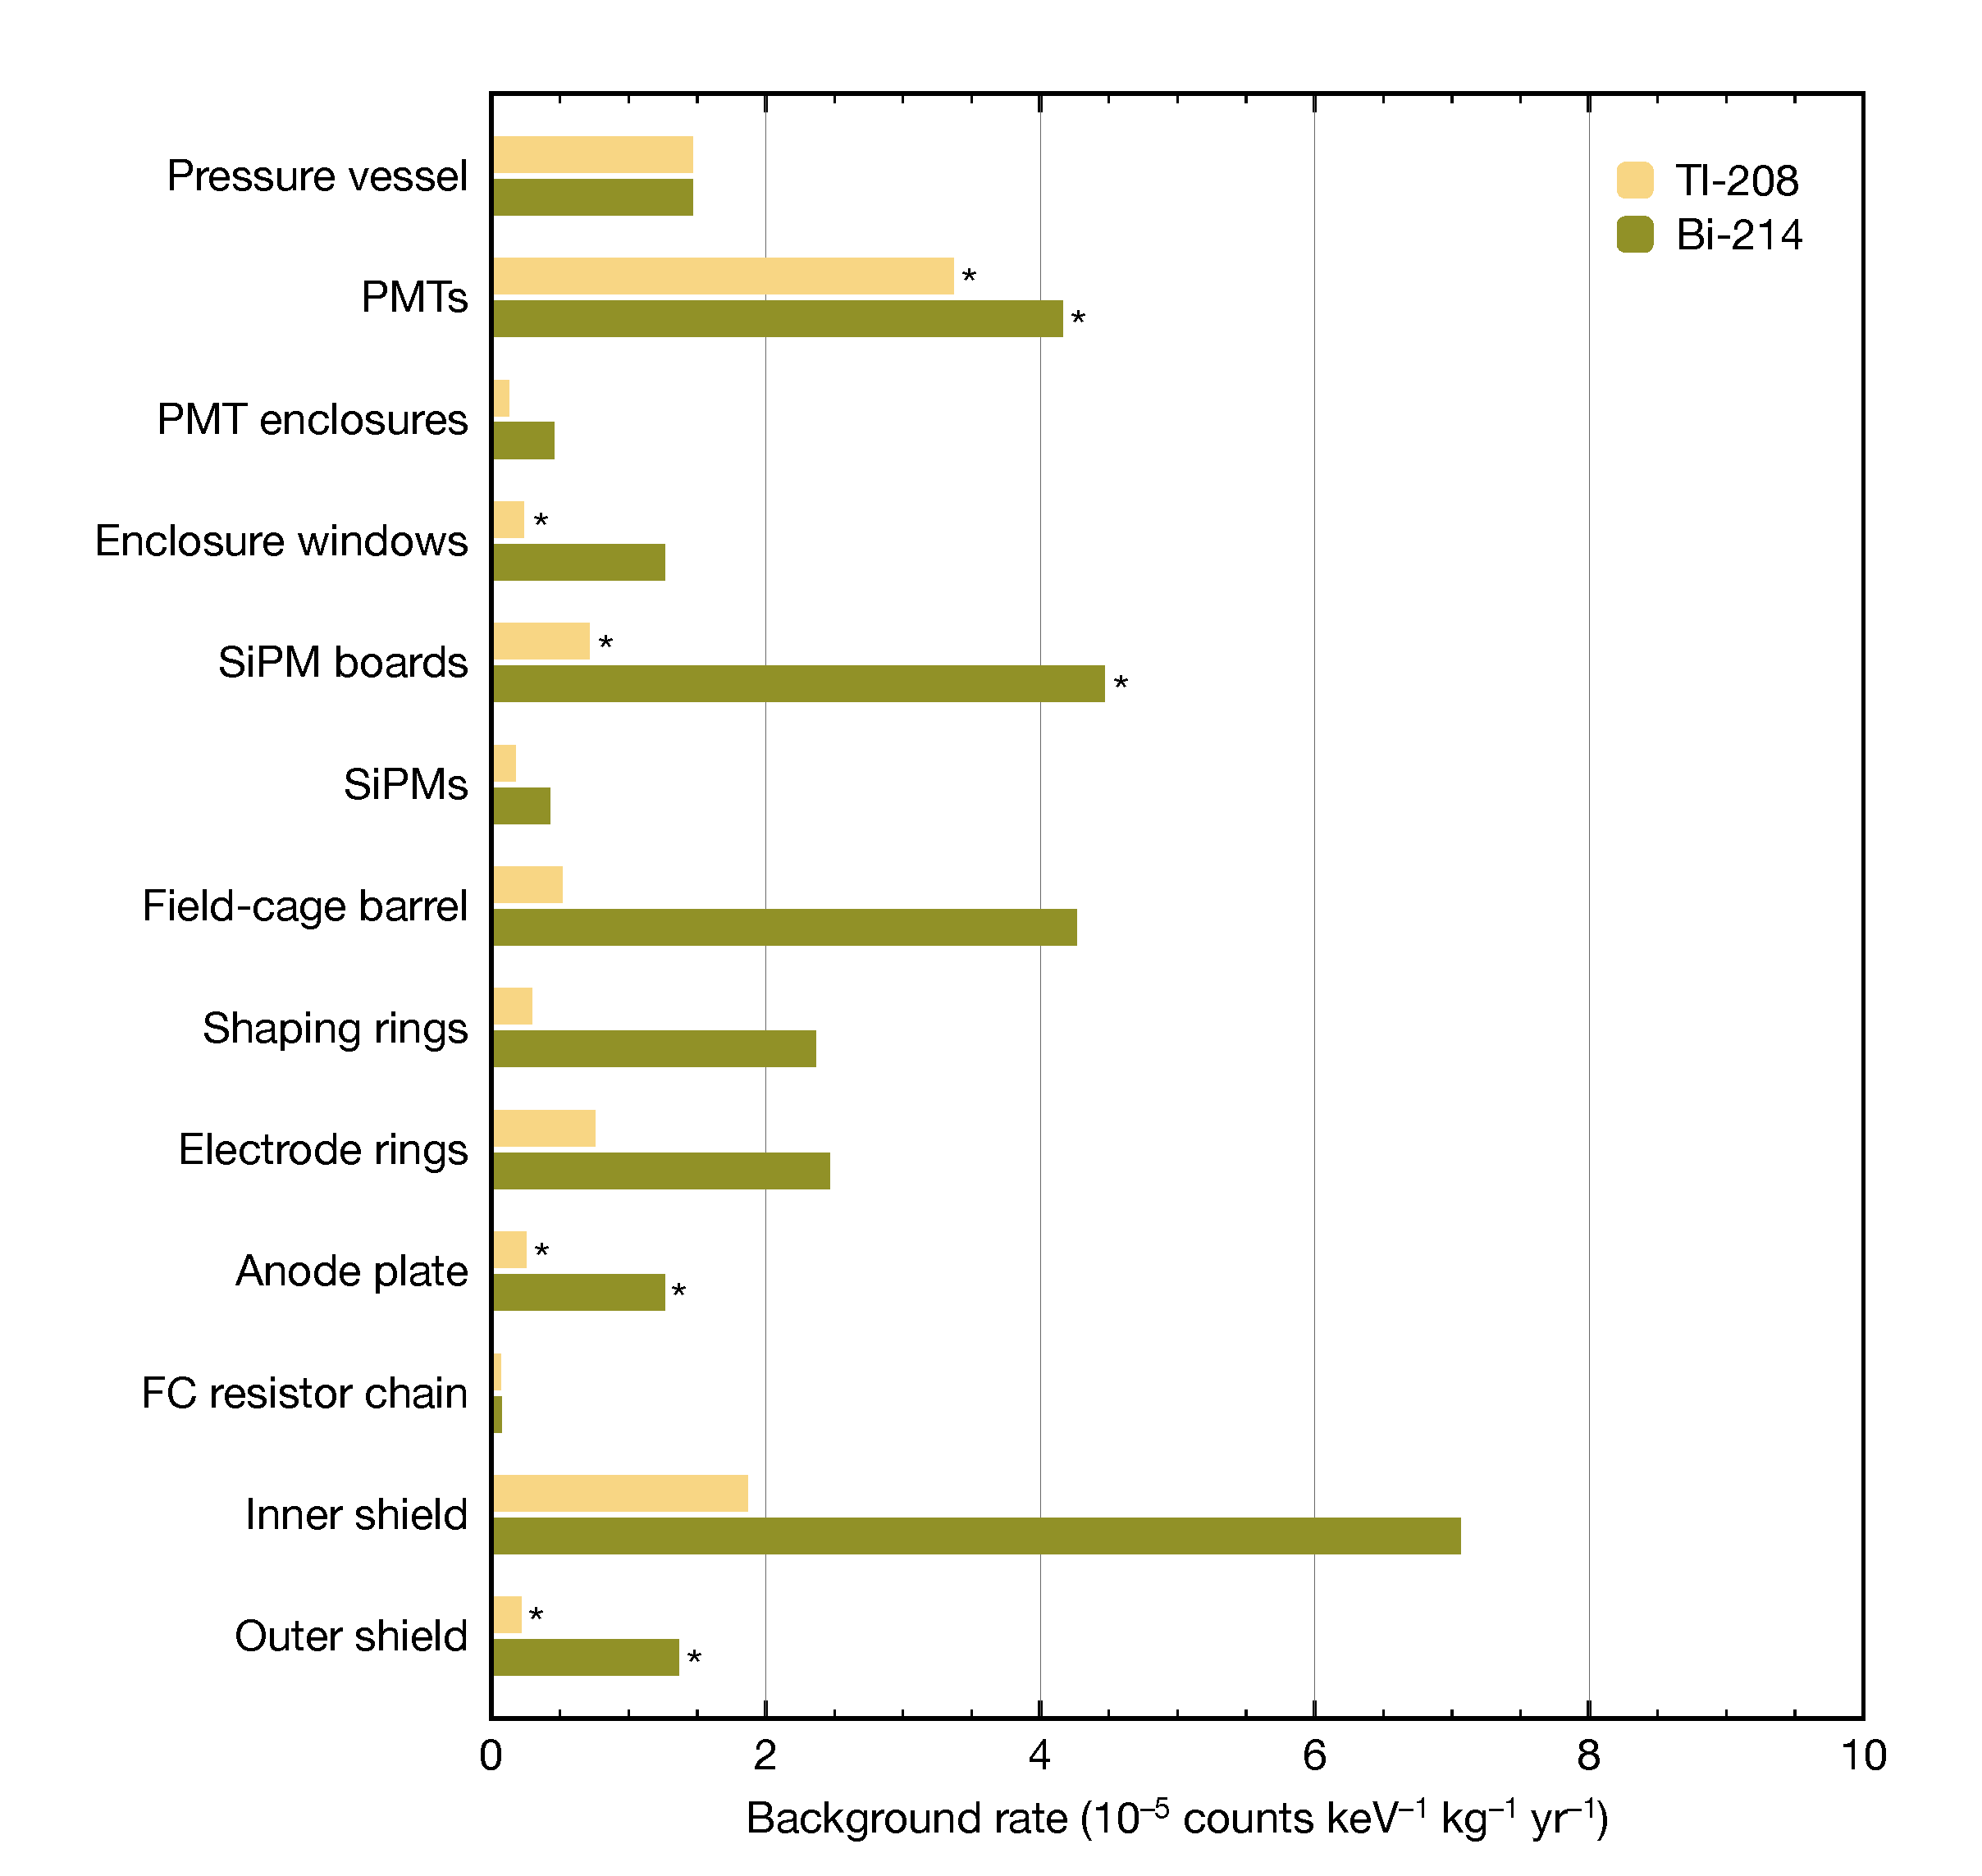
\includegraphics[scale=0.25]{radiobudget.png}
%
%\column{0.50\textwidth}
%$\bullet~$ Leading suspects: ICS (last shield), sensors (PMTs and SiPMs) and Field Cage (resistors).  
%
%$\bullet~$ Caveats. Radioactive budget comes from measuring individual components (labeled with *), some times using limits, and some times assuming uniformity (\url{https://arxiv.org/pdf/1511.09246}).
%
%$\bullet~$ The only way to understand (and improve) the radioactive budget of NEXT-100 is to assemble and operate the detector. 
% \end{columns}
%\end{frame}
%
%\begin{frame}{NEXT-100 Radioactive Budget}
%\begin{columns}
%\column{0.50\textwidth}
%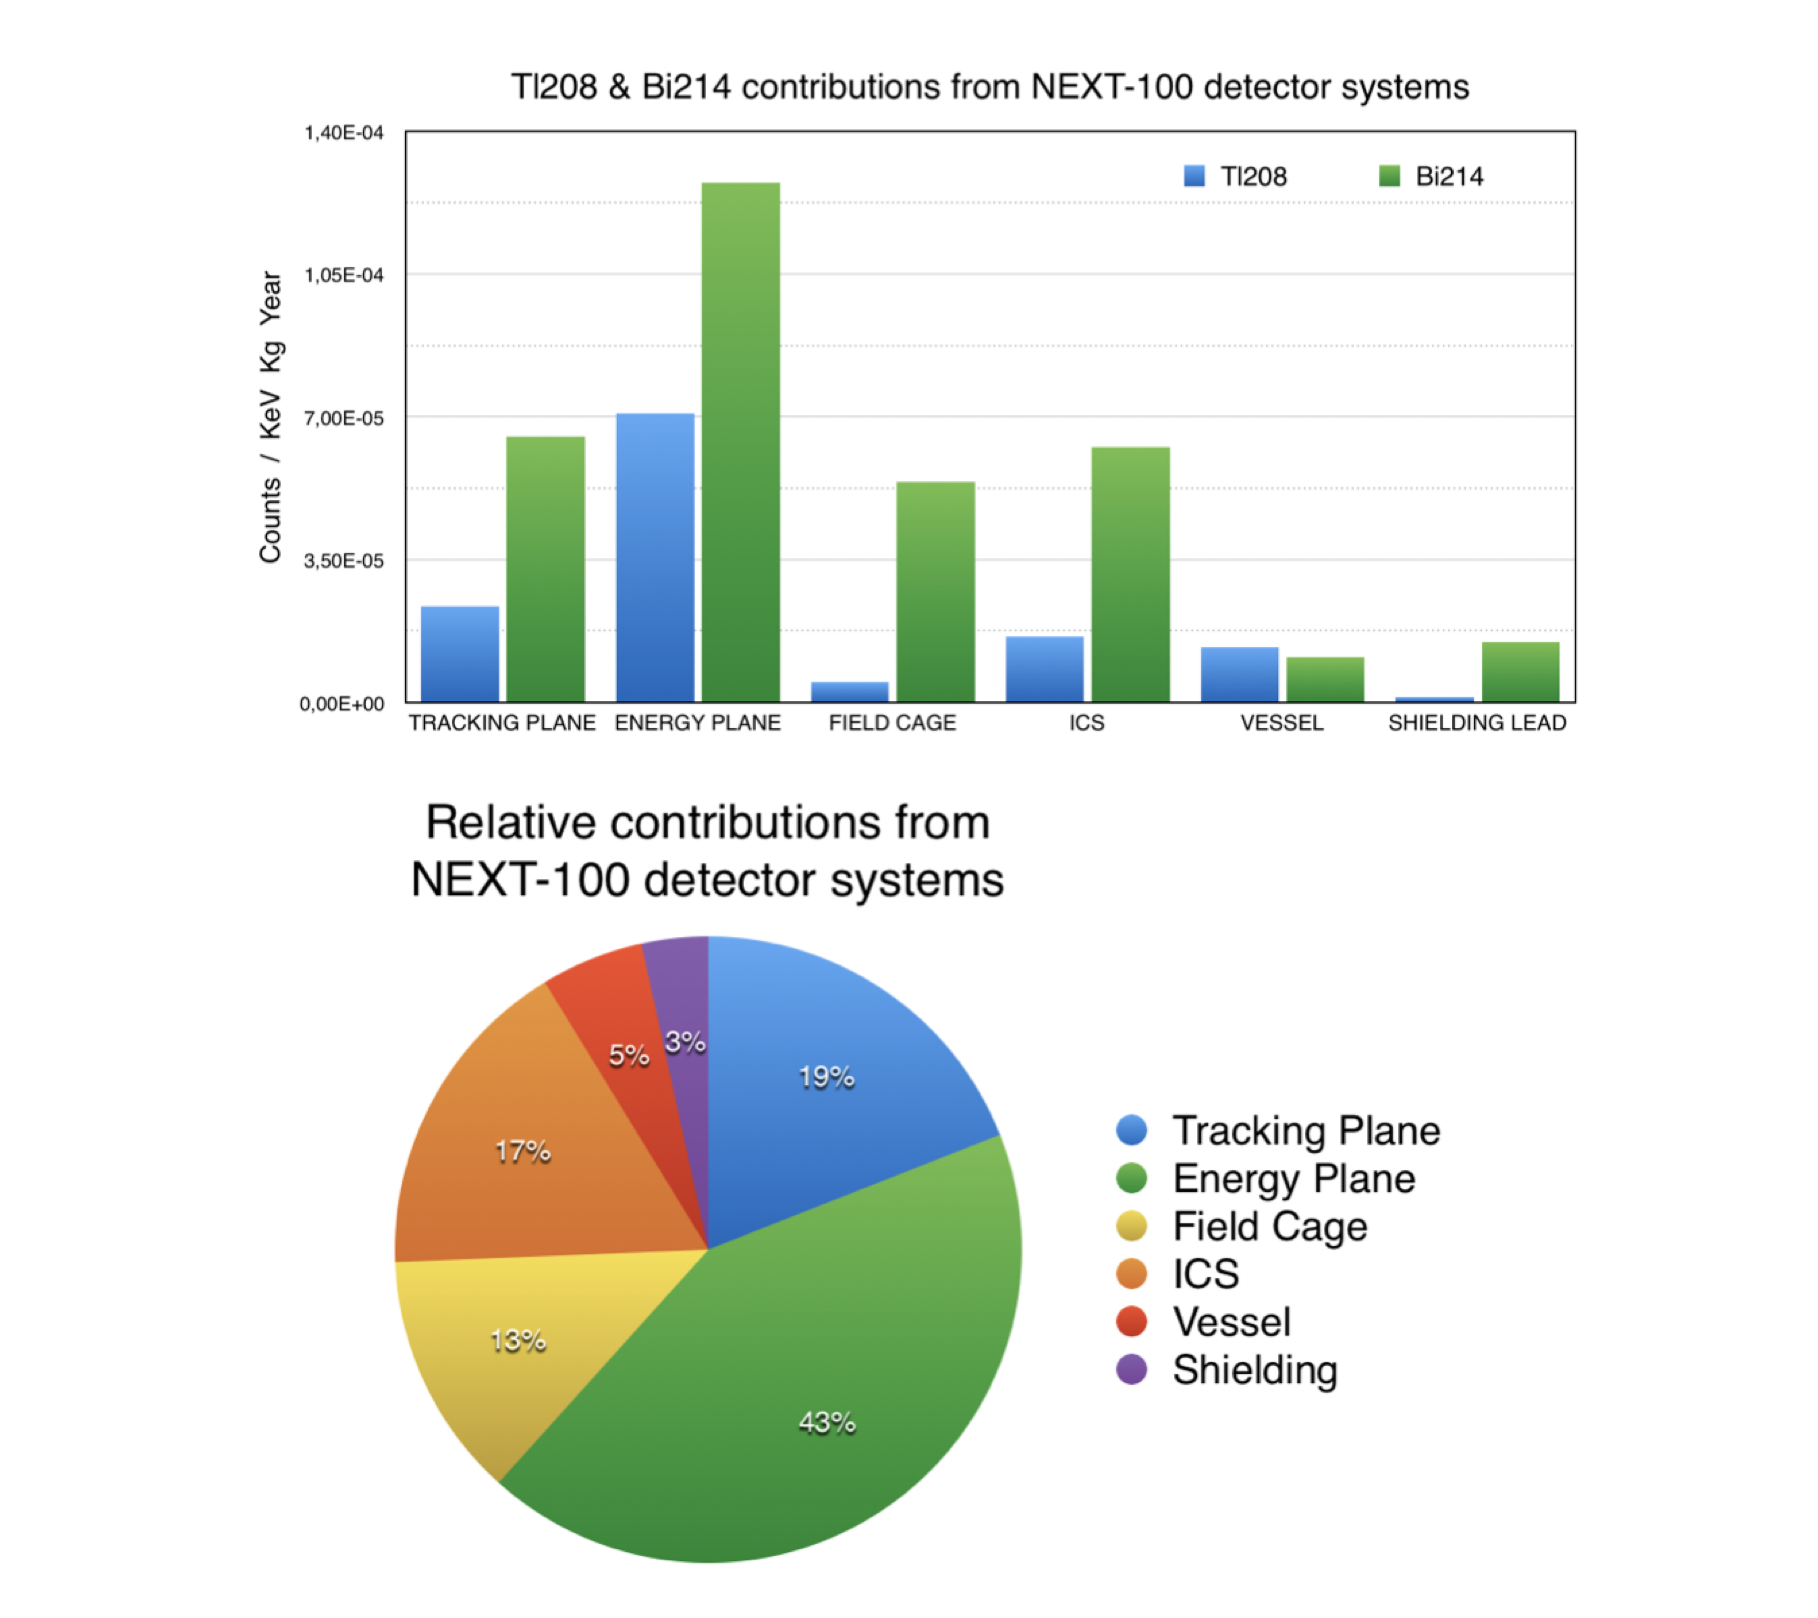
\includegraphics[scale=0.25]{budgetPie.png}
%
%\column{0.50\textwidth}
%$\bullet~$ Leading suspects: ICS (last shield), sensors (PMTs and SiPMs) and Field Cage (resistors).  
%
%$\bullet~$ Caveats. Radioactive budget comes from measuring individual components (labeled with *), some times using limits, and some times assuming uniformity (\url{https://arxiv.org/pdf/1511.09246}).
%
%$\bullet~$ The only way to understand (and improve) the radioactive budget of NEXT-100 is to assemble and operate the detector. 
% \end{columns}
%\end{frame}
%
%
%
%\begin{frame}{Specific Activities}
%\begin{columns}
%\column{0.70\textwidth}
%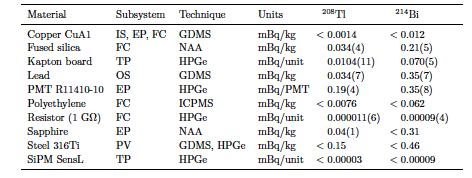
\includegraphics[scale=0.60]{specificActivities.png}
%
%\column{0.30\textwidth}
%$\bullet~$ Some of the specific activities in table may vary depending on the supplier and the manufacturing process. Two leading examples are copper and steel, which can vary up to an order of magnitude.  
%
%$\bullet~$ Other components (like PMTs) are very well known (but unavoidable, unless you get rid of them). 
%
% \end{columns}
%\end{frame}

%%%%

%\begin{frame}{Radioactive Budget}
%\begin{columns}
%\column{0.70\textwidth}
%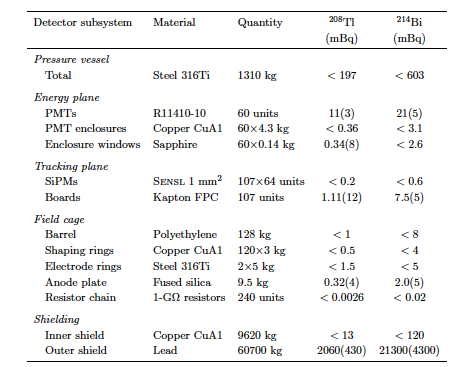
\includegraphics[scale=0.60]{rbudget.png
%}
%
%\column{0.30\textwidth}
%$\bullet~$ Radioactive budget depends on the mass of the material, its specific activity and whether is shielded or not.  
%
%$\bullet~$ Por instante, the PV and the LC would contribute with a huge amount if not shielded by the ICS. 
%
%$\bullet~$ Leading components are the PMTs and the ICS.  
%
% \end{columns}
%\end{frame}

%%%
%\begin{frame}{Detector's acceptance}
%\begin{columns}
%\column{0.55\textwidth}
%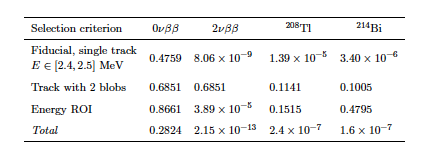
\includegraphics[scale=0.58]{acceptance.png
%}
%
%\column{0.45\textwidth}
%$\bullet~$ Leading effect: Single track in fiducial volume (and wide ROI) yields a background suppression of $\sim 1.4 \times 10^{-5}$~(\TL) and $\sim 3.4 \times 10^{-6}$~(\BI), with a signal efficiency of $\sim$ 68 \%.   
%
%$\bullet~$ Topological signature and improved ROI add one order of magnitude each for \TL\ (worse for \BI\ which is closer to \qbb) for a total rejection of   $\sim 2.4 (1.6) \times 10^{-7}$~ and a signal efficiency of $\sim$ 28\%. 
%
%$\bullet~$ The combined rejection power of the topological signal is $\sim 10^{-7}$, but the separation between one and two electrons, ``only'', 10\%. 
%
% \end{columns}
%\end{frame}

\begin{frame}{Background rate: discussion}
%\begin{columns}
%\column{0.55\textwidth}
%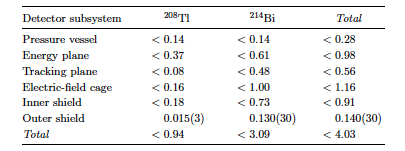
\includegraphics[scale=0.58]{finalContributions.png}
%
%\column{0.45\textwidth}
$\bullet~$ Radioactive background contributes with 0.92 cts/yr.  However, uncertainty are (very large) since all leading components are upper limits. The only way to understand better this background is to operate the NEXT-100 detector, fit the background model to the data and find the leading contributions.  

$\bullet~$ Contribution of $\mu$ induced background is 0.28 cts/yr. It can be reduced operating at a deeper location, but not dominant.  
 

% \end{columns}
\end{frame}

\begin{frame}{Background rate extrapolating NEXT-100 at the ton scale}
\begin{columns}
\column{0.50\textwidth}
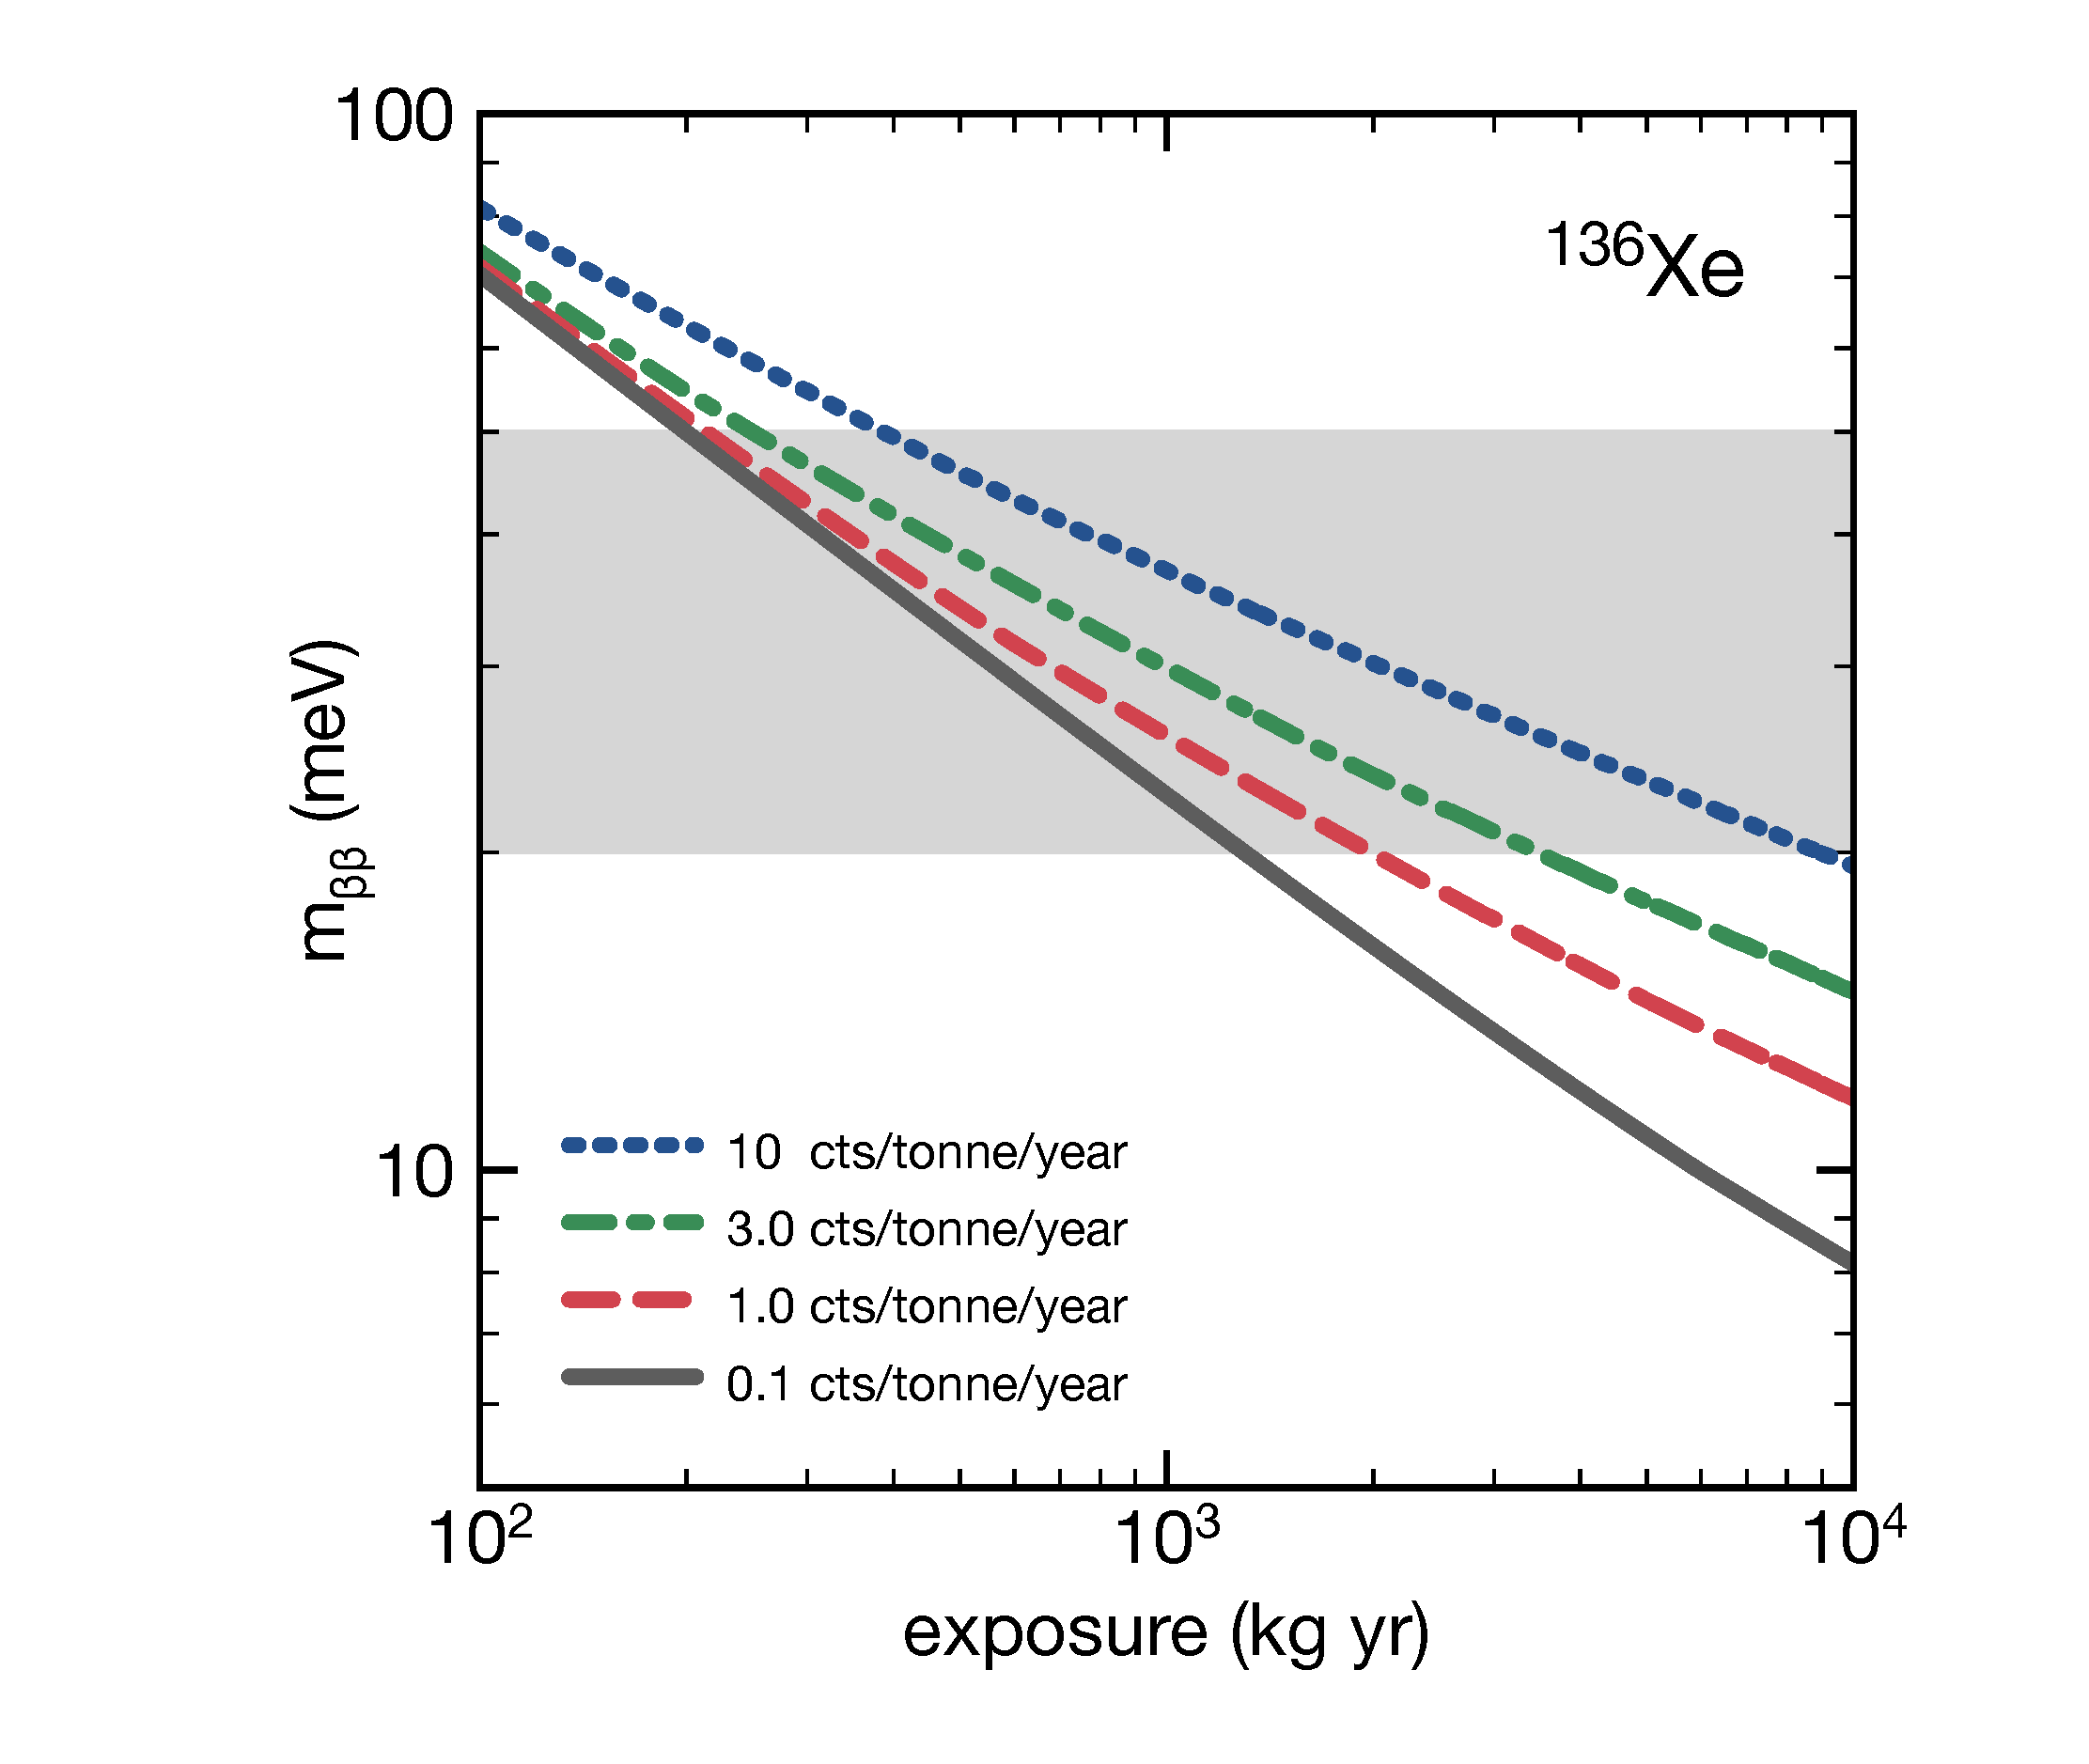
\includegraphics[scale=0.28]{sensiXe.png}

\column{0.50\textwidth}

\[
n_{ton}^{yr} \sim 12 {\rm ~events}
\]
$\bullet~$ {\bf Not good enough!} With 12 events per year and tonne in the ROI we would need 10 years for 1 ton detector with perfect efficiency (30 years for 1 ton detector with 30\% efficiency as NEXT). We need to reduce the total background in the ROI but at least one order of magnitude. How?

\end{columns}
\end{frame}

\begin{frame}{NEXT-HD}
\begin{columns}
\column{0.50\textwidth}
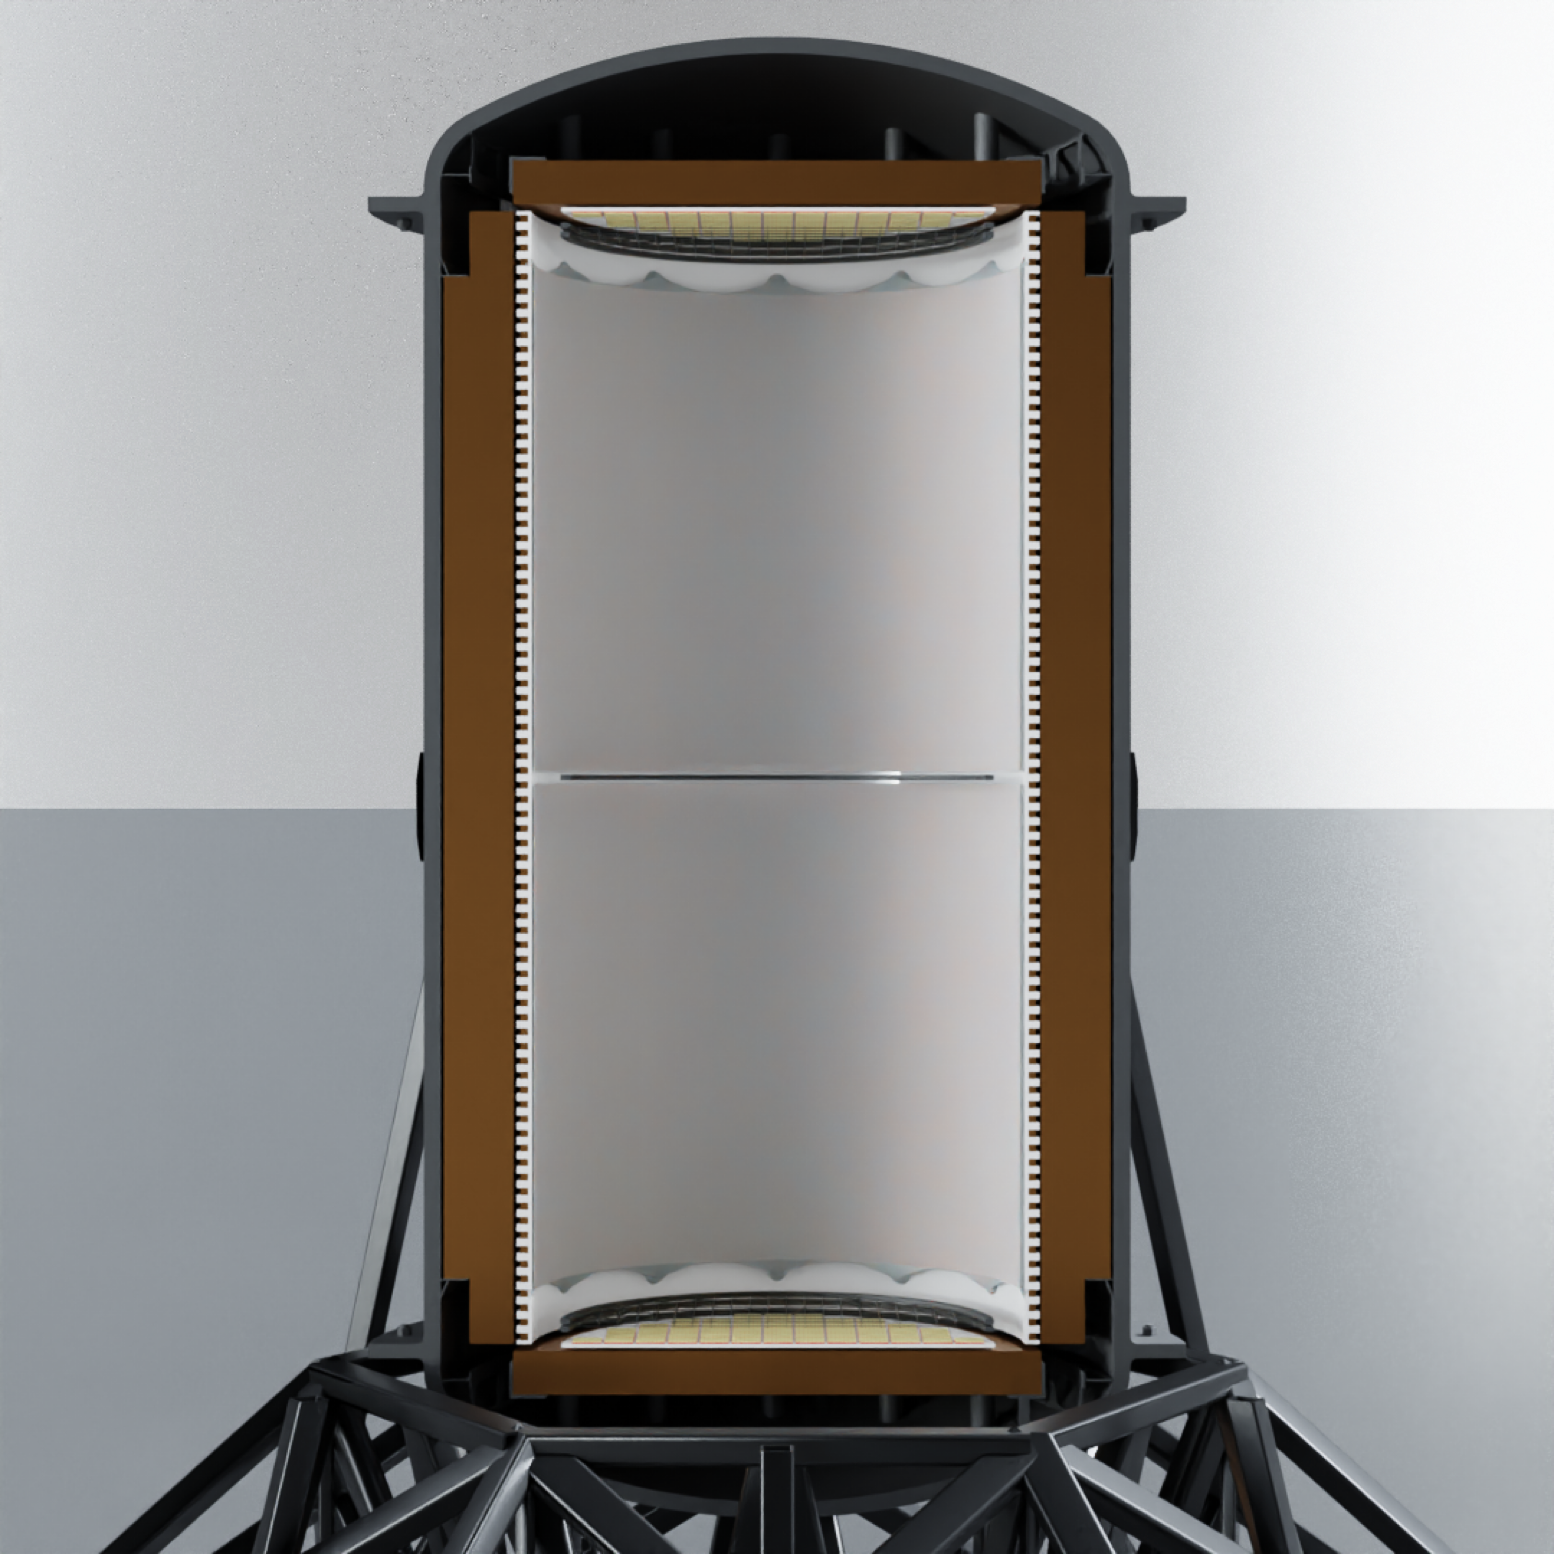
\includegraphics[scale=0.28]{nextHD.png}

\column{0.50\textwidth}

$\bullet~$ {\bf Scale up dimensions}: A symmetric detector of $2 \times 1.5$~m length and $2.2$~m diameter, ``doubling size of NEXT-100'',  holds 1 tonne at 15 bar and allows operational voltages in the same range than those used by NEXT-100 (thus, minimising risk).

$\bullet~$ {\bf Eliminate PMTs}, which introduce a substantial background and are difficult to operate at high pressure (also, PMTs do not allow a symmetric detector). 

$\bullet~$ {\bf Vertical orientation} simplifies mechanics. 

\end{columns}
\end{frame}

\begin{frame}{Barrel Fiber Detector}
\begin{columns}
\column{0.50\textwidth}
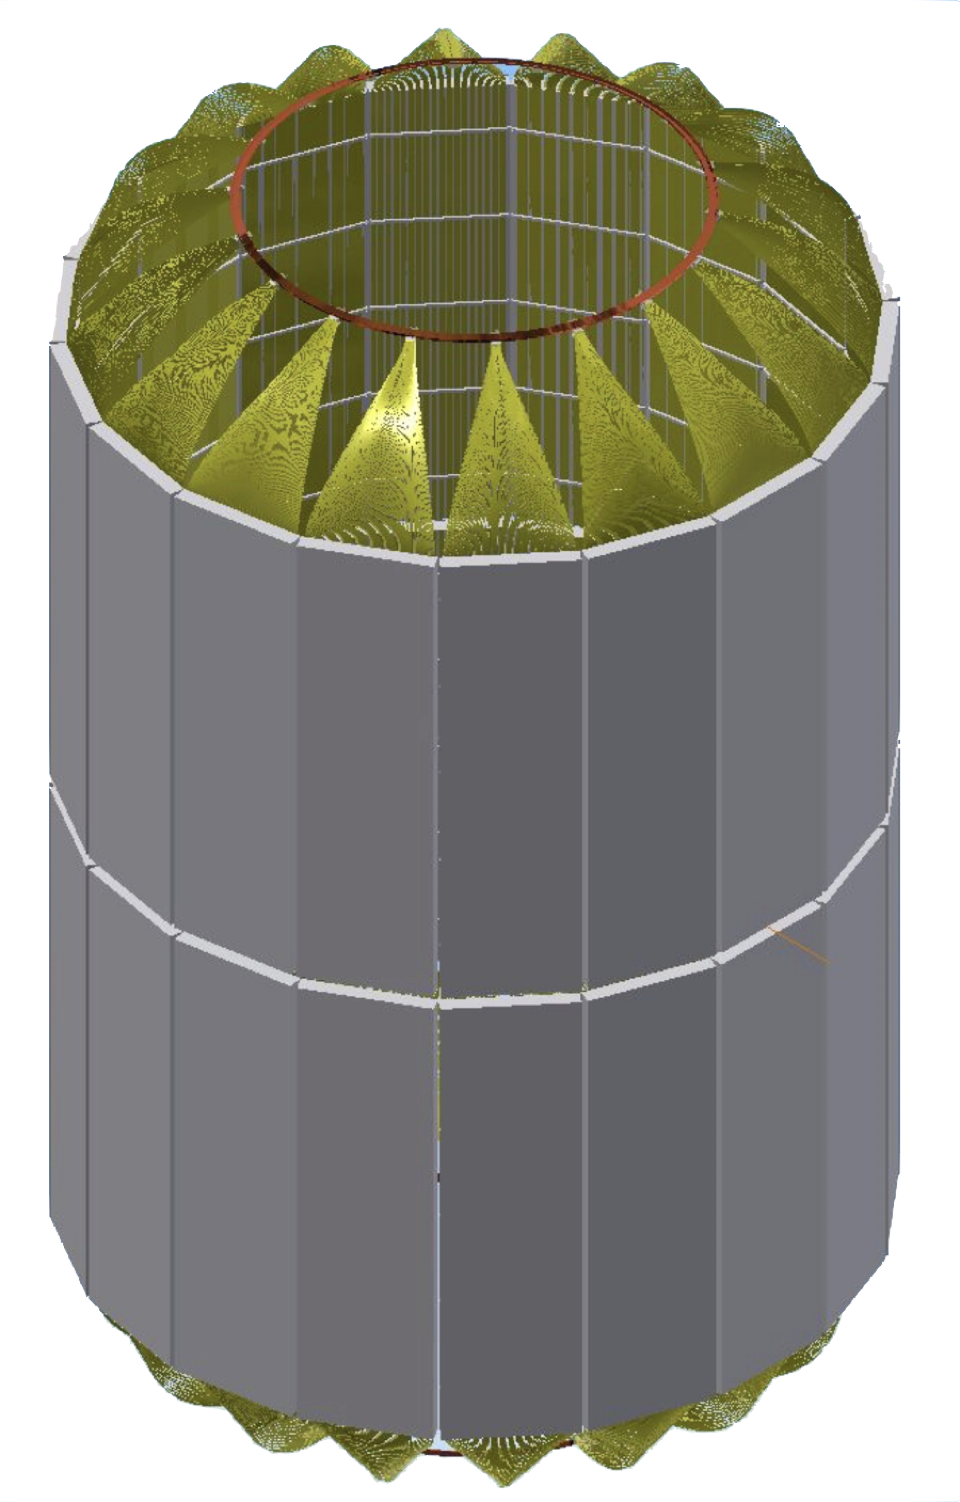
\includegraphics[scale=0.28]{cad.png}

\column{0.50\textwidth}

$\bullet~$ Measure the energy and \so\ with a Barrel Fibre Detector, read out by (cooled) SiPMs.

$\bullet~$ Reduces background budget, simplifies mechanics and should allow improve energy resolution (smoother energy map). Improve energy resolution reduces all backgrounds. With 0.5\% FWHM, most backgrounds are reduced by a factor 2 and \BI\ by a factor 4. 

\end{columns}
\end{frame}

\begin{frame}{Use Xe/He mixtures}
\begin{columns}
\column{0.50\textwidth}
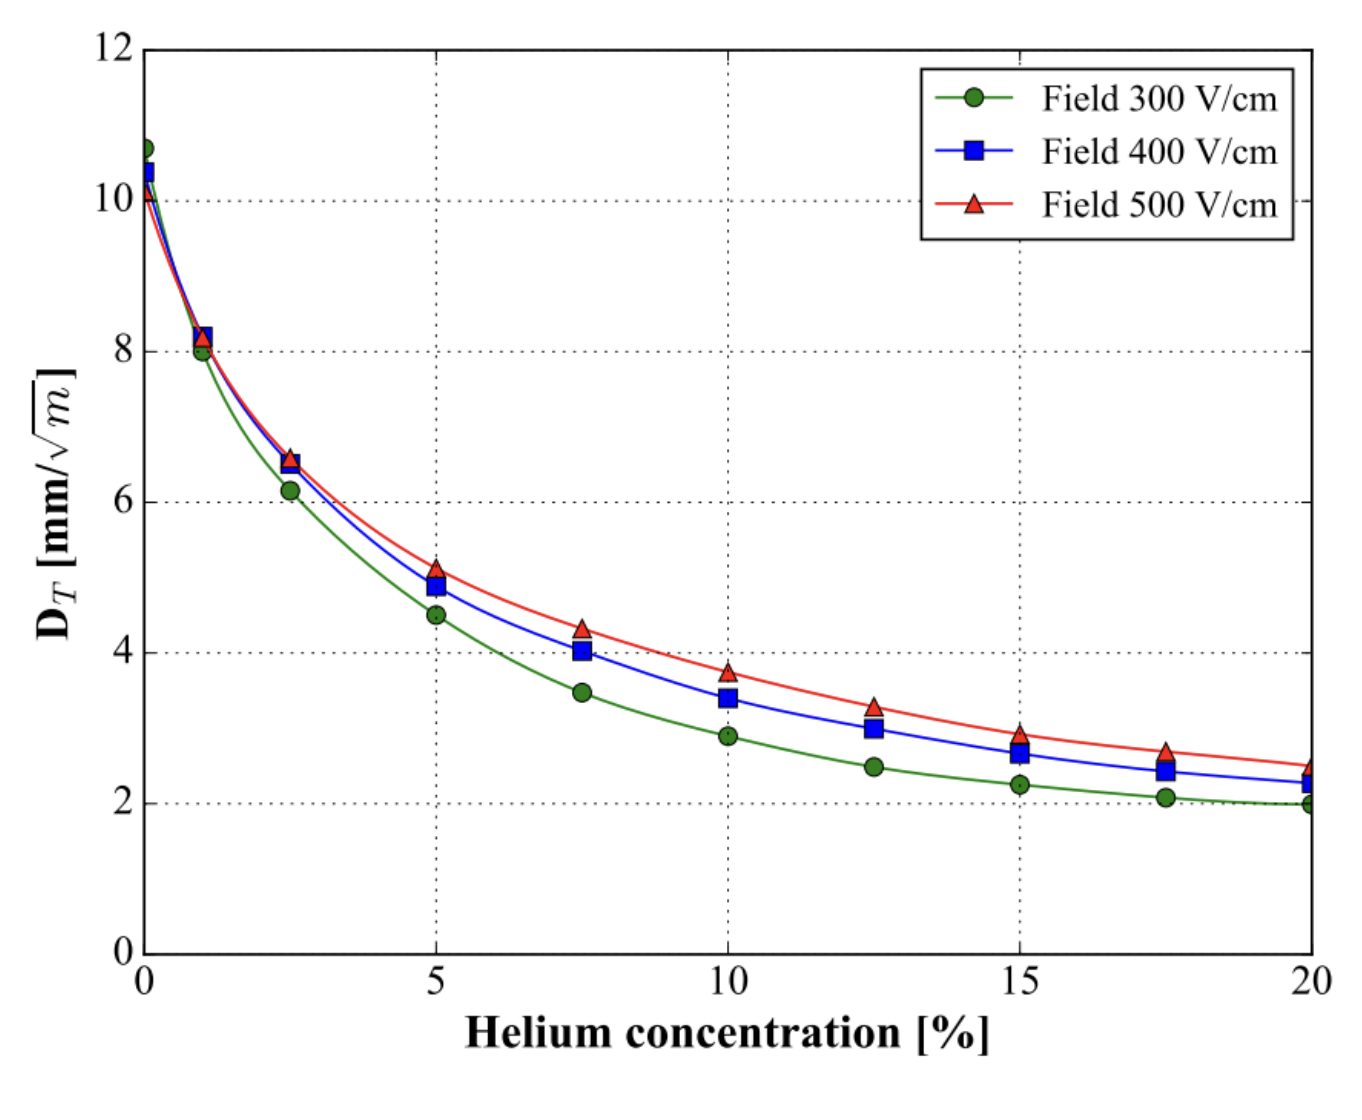
\includegraphics[scale=0.15]{xeHe.png}

\column{0.50\textwidth}

$\bullet~$ Reduces transverse diffusion by a factor 5 (thus the name, ``High Definition" NEXT).

$\bullet~$ Combined with topology reconstruction with DNNs, should allow improving background rejection by a factor 2-3. 

$\bullet~$ Addition of ${}^{3}He$ (high rate of capture of neutrons, 0.1 \% is enough) or deeper location to reduce the impact of \XES. 

$\bullet~$ Deeper location also suppresses $\mu$ induced background. 

\end{columns}
\end{frame}

\begin{frame}{Backgrounds in NEXT-HD}
\begin{columns}
\column{0.60\textwidth}
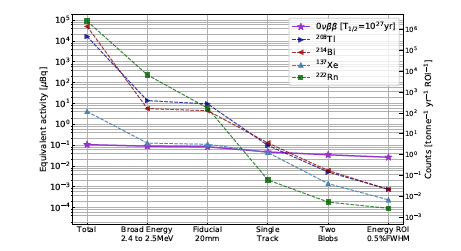
\includegraphics[scale=0.40]{bkgndHD.png}
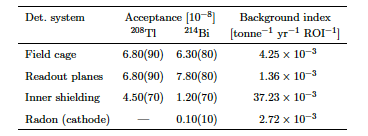
\includegraphics[scale=0.40]{RadioHD.png}


\column{0.40\textwidth}

$\bullet~$ \TL\ and \BI\ contribute in the same amount. Dominant contribution is the ICS. R\&D to produce large amounts of ultra-pure radioactive copper is a must. 

$\bullet~$ Deeper location to reduce non-radioactive backgrounds. \XES\ becomes subdominant if operating at LNGS (negligible at SNOLAB) 

$\bullet~$ According to simulations a background rate below 1 cts/yer in the ROI can be achieved. 

\end{columns}
\end{frame}



%nextHD.png
%hdWithFibers.png
%xeHe.png
%smfPhysRev.png

%cad.png

\begin{frame}{Sailing to Ithaca}
\begin{columns}
\column{0.50\textwidth}
\includegraphics[scale=0.18]{francesDemo.png}

Francesc (then grad student) working in NEXT-DEMO, circa 2012

\column{0.50\textwidth}
\includegraphics[scale=0.17]{FrancescNew.png}

Francesc (now NEXT TC) in NEXT-White, circa 2022
 
 \end{columns}
\end{frame}









%%%
\end{document}